\section{process creation and management}

\begin{frame}<1>[label=posixProcessFunctions]{POSIX process management}
\begin{itemize}
\item essential operations
\vspace{.5cm}
\item process information: \myemph<2>{\texttt{getpid}}
\item process creation: \myemph<3>{\texttt{fork}}
\item running programs: \myemph<4>{\texttt{exec*}}
\begin{itemize}
\item {\fontsize{9}{10}\selectfont also \texttt{posix\_spawn} (not widely supported), \ldots}
\end{itemize}
\item waiting for processes to finish: \texttt{\myemph<5>{waitpid}} {\small (or \texttt{\myemph<5>{wait}})}
\item process destruction, `signaling': \texttt{exit}, \texttt{kill}
\end{itemize}
\end{frame}



\againframe<3>{posixProcessFunctions}


\usetikzlibrary{matrix,patterns,arrows.meta,decorations.pathreplacing}
\begin{frame}{\texttt{fork}}
\begin{itemize}
\item \texttt{pid\_t fork()} --- copy the current process
\item returns twice:
    \begin{itemize}
    \item in \textit{parent} (original process): pid of new \textit{child} process
    \item in \textit{child} (new process): \texttt{0}
    \end{itemize}
\item \myemph{everything (but pid) duplicated} in parent, child:
    \begin{itemize}
    \item memory
    \item file descriptors (later)
    \item registers
    \end{itemize}
\end{itemize}
\end{frame}


\usetikzlibrary{matrix,patterns,arrows.meta,decorations.pathreplacing}

% FIXME: fork process control block image

\begin{frame}[label=forkPCBs]{fork and process info (w/o copy-on-write)}
\begin{tikzpicture}
\tikzset{
    pcb/.style={
        tight matrix,
        column 1/.style={nodes={draw,thin,text width=3.0cm,font=\small,minimum height=0.4cm}},
        column 2/.style={nodes={draw,thin,text width=5.5cm,font=\fontsize{9}{10}\tt\selectfont,minimum height=0.4cm}},
    },
    page/.style={
        draw,thick,
        pattern=north west lines,
        minimum width=2cm,
        node contents={~},
    },
    pointer/.style={
        draw,very thick,-Latex,
    },
    pointer light/.style={
        draw,thick,-Latex,
    },
    tall/.style={
        minimum height=0.85cm
    },
    one pt/.style={
        fill=blue!40,
    },
    one pt line/.style={
        draw=blue!80!black,
    },
    one memory/.style={
        fill=green!40,
    },
    one memory line/.style={
        draw=green!80!black,
    },
    two pt/.style={
        fill=orange!40,
    },
    two pt line/.style={
        draw=orange!80!black,
    },
    two memory/.style={
        fill=violet!40,
        alt=<1-2>{one memory},
    },
    two memory line/.style={
        draw=violet!80!black,
        alt=<1-2>{one memory line},
    },
    fork line/.style={
        draw=black!30,line width=2mm,-{Latex[length=6mm]}
    },
}
\matrix[pcb,label={[font=\small]north:parent process info}] (proc one) {
    |[tall]| user regs \&
    |[tall]|
    {rax {\fontsize{8}{9}\selectfont (return val.)}=\sout<5->{42}\only<5->{\textit{\myemph<5>{child pid}}}, \\ rcx=133,} \ldots \\
    memory mapping \& |[one pt]| ~ \\
    |[tall]| open files \& |[tall]| {fd 0: \ldots \\ fd 1: \ldots } \\
    \ldots \& \ldots \\
};
\newcommand{\halfvthick}{.2mm}
\node[draw,very thick,pattern=north west lines,minimum width=2cm,minimum height=6cm,anchor=north west,
    label={north:memory}] (memory) at ([xshift=1.5cm,yshift=0cm]proc one.north east) {};
\foreach \y in {-1.8cm} {
    \draw[very thick,one pt] ([yshift=\y,xshift=\halfvthick]memory.north west) rectangle ++ (2cm,-1mm);
}
\coordinate (one pt root) at ([yshift=-1.8cm-0.5mm,xshift=\halfvthick]memory.north west);
\draw[pointer light,one pt line] (proc one-2-2.east) -- ++(.25cm,0cm) |- ([yshift=-1.8cm]memory.north west);
\draw[pointer light,one memory line] (one pt root) -- ++(-.5cm,0cm) |- ([yshift=-0.9cm]memory.north west);
\draw[pointer light,one memory line] (one pt root) -- ++(-.5cm,0cm) |- ([yshift=-1.1cm]memory.north west);
\draw[pointer light,one memory line] (one pt root) -- ++(-.5cm,0cm) |- ([yshift=-1.5cm]memory.north west);
\foreach \y in {-0.9cm,-1.1cm,-1.5cm} {
    \draw[very thick,one memory] ([yshift=\y,xshift=\halfvthick]memory.north west) rectangle ++ (2cm,-1mm);
}
\begin{visibleenv}<2->
\matrix[pcb,anchor=north west,label={[font=\small]north:child process info}] (proc two) at ([yshift=-1cm]proc one.south west) {
    |[tall]| user regs \&
    |[tall]|
    {rax {\fontsize{8}{9}\selectfont(return val.)}=\sout<5->{42}\only<5->{\myemph<5>{0}}, \\ rcx=133, \ldots} \\
    memory mapping \& |[two pt]| ~ \\
    |[tall]| open files \& |[tall]| {fd 0: \ldots \\ fd 1: \ldots } \\
    \ldots \& \ldots \\
};
\draw[fork line] ([xshift=-0.25cm]proc one.west) -- ++(-1cm,0cm) |- ([xshift=-0.25cm]proc two.west)
    node[pos=0.25,right] {copy};
\end{visibleenv}
\begin{visibleenv}<3->
\foreach \y in {-4.3cm} {
    \draw[very thick,two pt] ([yshift=\y,xshift=\halfvthick]memory.north west) rectangle ++ (2cm,-1mm);
}
\coordinate (two pt root) at ([yshift=-4.3cm-0.5mm,xshift=\halfvthick]memory.north west);
\draw[pointer light,two pt line] (proc two-2-2.east) -- ++(.25cm,0cm) |- ([yshift=-4.3cm]memory.north west);
\draw[pointer light,two memory line] (two pt root) -- ++(-.75cm,0cm) |- ([yshift=-4.4cm]memory.north west);
\draw[pointer light,two memory line] (two pt root) -- ++(-.75cm,0cm) |- ([yshift=-4.6cm]memory.north west);
\draw[pointer light,two memory line] (two pt root) -- ++(-.75cm,0cm) |- ([yshift=-4.7cm]memory.north west);
\foreach \y in {-4.4cm,-4.6cm,-4.7cm} {
    \draw[very thick,two memory] ([yshift=\y,xshift=\halfvthick]memory.north west) rectangle ++ (2cm,-1mm);
}
\draw[fork line] ([yshift=-1.4cm,xshift=.5cm]memory.north east) coordinate (one memory)-- ++(1cm, 0cm) |- ([yshift=-4.6cm,xshift=.5cm]memory.north east) coordinate (two memory)
    node[pos=0.25,left] {copy};
\draw[ultra thick,decorate,decoration={brace,mirror}] ([xshift=-.25cm,yshift=-6mm]one memory) -- ([xshift=-.25cm,yshift=6mm]one memory);
\draw[ultra thick,decorate,decoration={brace,mirror}] ([xshift=-.25cm,yshift=-6mm]two memory) -- ([xshift=-.25cm,yshift=6mm]two memory);
\end{visibleenv}
\end{tikzpicture}
\end{frame}

%\usetikzlibrary{matrix,patterns,arrows.meta,decorations.pathreplacing}

\begin{frame}[label=forkCows]{fork (w/ copy-on-write, if parent writes first)}
\begin{tikzpicture}
\tikzset{
    pcb/.style={
        tight matrix,
        column 1/.style={nodes={draw,thin,text width=2.5cm,font=\small,minimum height=0.4cm}},
        column 2/.style={nodes={draw,thin,text width=5.5cm,font=\fontsize{9}{10}\tt\selectfont,minimum height=0.4cm}},
    },
    page/.style={
        draw,thick,
        pattern=north west lines,
        minimum width=2cm,
        node contents={~},
    },
    pointer/.style={
        draw,very thick,-Latex,
    },
    pointer light/.style={
        draw,thick,-Latex,
    },
    tall/.style={
        minimum height=0.85cm
    },
    one pt/.style={
        fill=blue!40,
    },
    one pt line/.style={
        draw=blue!80!black,
    },
    one memory/.style={
        fill=green!40,
    },
    shared memory/.style={
        fill=yellow!40,
    },
    one memory line/.style={
        draw=green!80!black,
    },
    one memory line cow/.style={
        draw=green!80!black,
        dashed,
    },
    two pt/.style={
        fill=orange!40,
    },
    two pt line/.style={
        draw=orange!80!black,
    },
    two memory/.style={
        fill=violet!40,
    },
    two memory line/.style={
        draw=violet!80!black,
    },
    two memory line cow/.style={
        draw=violet!80!black,
        dashed 
    },
    fork line/.style={
        draw=black!30,line width=2mm,-{Latex[length=6mm]}
    },
}
\matrix[pcb,label={[font=\small]north:parent process info}] (proc one) {
    |[tall]| user regs \&
    |[tall]|
    {rax {\fontsize{8}{9}\selectfont (return val.)}=\sout<1->{42}\only<1->{\textit{\myemph<5>{child pid}}}, \\ rcx=133,} \ldots \\
    page tables \& |[one pt]| ~ \\
    |[tall]| open files \& |[tall]| {fd 0: \ldots \\ fd 1: \ldots } \\
    \ldots \& \ldots \\
};
\newcommand{\halfvthick}{.2mm}
\node[draw,very thick,pattern=north west lines,minimum width=2cm,minimum height=6cm,anchor=north west,
    label={north:memory}] (memory) at ([xshift=1.5cm,yshift=0cm]proc one.north east) {};
\foreach \y in {-1.8cm} {
    \draw[very thick,one pt] ([yshift=\y,xshift=\halfvthick]memory.north west) rectangle ++ (2cm,-1mm);
}
\coordinate (one pt root) at ([yshift=-1.8cm-0.7mm,xshift=\halfvthick]memory.north west);
\draw[pointer light,one pt line] (proc one-2-2.east) -- ++(.25cm,0cm) |- ([yshift=-1.8cm]memory.north west);
\begin{visibleenv}<1>
\draw[pointer light,one memory line] (one pt root) -- ++(-.5cm,0cm) |- ([yshift=-0.4cm]memory.north west);
\draw[pointer light,one memory line] (one pt root) -- ++(-.6cm,0cm) |- ([yshift=-1.1cm]memory.north west);
\draw[pointer light,one memory line] (one pt root) -- ++(-.7cm,0cm) |- ([yshift=-1.5cm]memory.north west);
\end{visibleenv}
\begin{visibleenv}<2>
\draw[pointer light,one memory line cow] (one pt root) -- ++(-.5cm,0cm) |- ([yshift=-0.4cm]memory.north west);
\end{visibleenv}
\begin{visibleenv}<3->
\draw[pointer light,one memory line,alt=<3>{red,very thick}] (one pt root) -- ++(-.5cm,0cm) |- ([yshift=-2.9cm]memory.north west);
\end{visibleenv}
\begin{visibleenv}<2->
\draw[pointer light,one memory line cow] (one pt root) -- ++(-.6cm,0cm) |- ([yshift=-1.1cm]memory.north west);
\draw[pointer light,one memory line cow] (one pt root) -- ++(-.7cm,0cm) |- ([yshift=-1.5cm]memory.north west);
\end{visibleenv}
\begin{visibleenv}<1>
\foreach \y in {-0.4cm,-1.1cm,-1.5cm} {
    \draw[very thick,one memory] ([yshift=\y,xshift=\halfvthick]memory.north west) rectangle ++ (2cm,-1mm);
}
\end{visibleenv}
\begin{visibleenv}<2->
\foreach \y in {-0.4cm,-1.1cm,-1.5cm} {
    \draw[very thick,shared memory] ([yshift=\y,xshift=\halfvthick]memory.north west) rectangle ++ (2cm,-1mm);
}
\end{visibleenv}
\begin{visibleenv}<2>
\path ([yshift=-0.8cm,xshift=0cm]memory.north east) coordinate (base memory) node [right=0.5mm,align=left] {shared\\read-only};
\draw[ultra thick,decorate,decoration={brace,mirror}] ([xshift=.1cm,yshift=-7mm]base memory) -- ([xshift=.1cm,yshift=7mm]base memory);
\end{visibleenv}
\begin{visibleenv}<3-4>
\path ([yshift=-1.3cm,xshift=0cm]memory.north east) coordinate (base memory alt) node [right=0.5mm,align=left] {shared\\read-only};
\draw[ultra thick,decorate,decoration={brace,mirror}] ([xshift=.1cm,yshift=-3mm]base memory alt) -- ([xshift=.1cm,yshift=3mm]base memory alt);
\end{visibleenv}
\begin{visibleenv}<3->
\foreach \y in {-2.9cm} {
    \draw[very thick,one memory] ([yshift=\y,xshift=\halfvthick]memory.north west) rectangle ++ (2cm,-1mm);
}
\path[alt=<3>{red}] ([yshift=-2.9cm,xshift=0cm]memory.north east) coordinate (copied memory) node [inner sep=0mm,right=4mm,align=left] (copy label) {copied};
    \node[align=left,font=\small,anchor=north west,inner sep=0.5mm] at (copy label.south west) {for\\ parent's\\ write};
\draw[ultra thick,decorate,decoration={brace,mirror}] ([xshift=.1cm,yshift=-2mm]copied memory) -- ([xshift=.1cm,yshift=2mm]copied memory);
\end{visibleenv}
\begin{visibleenv}<4>
\path[alt=<4>{red}] ([yshift=-0.4cm,xshift=0cm]memory.north east) coordinate (now unshared memory) node[inner sep=0mm,right=0mm]{$\leftarrow$} node [inner sep=0mm,right=5mm,align=left,font=\small] {no longer\\shared};
\draw[ultra thick,decorate,decoration={brace,mirror}] ([xshift=.1cm,yshift=-2mm]copied memory) -- ([xshift=.1cm,yshift=2mm]copied memory);
\end{visibleenv}
\begin{visibleenv}<3>
\path[alt=<3>{red}] ([yshift=-0.4cm,xshift=0cm]memory.north east) coordinate (uncopied memory) node[inner sep=0mm,right=0mm]{$\leftarrow$} node [inner sep=0mm,right=5mm,align=left,font=\small] {on parent\\write};
\end{visibleenv}
\begin{visibleenv}<2->
\matrix[pcb,anchor=north west,label={[font=\small]north:child process info}] (proc two) at ([yshift=-1cm]proc one.south west) {
    |[tall]| user regs \&
    |[tall]|
    {rax {\fontsize{8}{9}\selectfont(return val.)}=\sout<1->{42}\only<1->{\myemph<5>{0}}, \\ rcx=133, \ldots} \\
    page tables\& |[two pt]| ~ \\
    |[tall]| open files \& |[tall]| {fd 0: \ldots \\ fd 1: \ldots } \\
    \ldots \& \ldots \\
};
\draw[fork line] ([xshift=-0.25cm]proc one.west) -- ++(-1cm,0cm) |- ([xshift=-0.25cm]proc two.west)
    node[pos=0.25,right] {copy};
\end{visibleenv}
\begin{visibleenv}<2->
\foreach \y in {-4.3cm} {
    \draw[very thick,two pt] ([yshift=\y,xshift=\halfvthick]memory.north west) rectangle ++ (2cm,-1mm);
}
\coordinate (two pt root) at ([yshift=-4.3cm-0.5mm,xshift=\halfvthick]memory.north west);
\draw[pointer light,two pt line] (proc two-2-2.east) -- ++(.25cm,0cm) |- ([yshift=-4.3cm]memory.north west);
\begin{visibleenv}<2->
\draw[pointer light,two memory line cow] (two pt root) -- ++(-.75cm,0cm) |- ([yshift=-0.45cm]memory.north west);
\draw[pointer light,two memory line cow] (two pt root) -- ++(-.75cm,0cm) |- ([yshift=-1.15cm]memory.north west);
\draw[pointer light,two memory line cow] (two pt root) -- ++(-.75cm,0cm) |- ([yshift=-1.55cm]memory.north west);
\end{visibleenv}
\begin{visibleenv}<0>
\draw[pointer light,two memory line] (two pt root) -- ++(-.75cm,0cm) |- ([yshift=-4.4cm]memory.north west);
\draw[pointer light,two memory line] (two pt root) -- ++(-.75cm,0cm) |- ([yshift=-4.6cm]memory.north west);
\draw[pointer light,two memory line] (two pt root) -- ++(-.75cm,0cm) |- ([yshift=-4.7cm]memory.north west);
\end{visibleenv}
\begin{visibleenv}<0>
\foreach \y in {-4.4cm,-4.6cm,-4.7cm} {
    \draw[very thick,two memory] ([yshift=\y,xshift=\halfvthick]memory.north west) rectangle ++ (2cm,-1mm);
}
\end{visibleenv}
% FIXME: XXX -----> = read-only marker
%\draw[fork line] ([yshift=-1.4cm,xshift=.5cm]memory.north east) coordinate (one memory)-- ++(1cm, 0cm) |- ([yshift=-4.6cm,xshift=.5cm]memory.north east) coordinate (two memory)
%    node[pos=0.25,left] {copy};
%\draw[ultra thick,decorate,decoration={brace,mirror}] ([xshift=-.25cm,yshift=-6mm]one memory) -- ([xshift=-.25cm,yshift=6mm]one memory);
%\draw[ultra thick,decorate,decoration={brace,mirror}] ([xshift=-.25cm,yshift=-6mm]two memory) -- ([xshift=-.25cm,yshift=6mm]two memory);
\end{visibleenv}
\end{tikzpicture}
\end{frame}
 % in backup

\begin{frame}{fork example}
\lstinputlisting[
    language=C,
    basicstyle=\sourcecodepro\fontsize{9}{10}\selectfont,
    moredelim={**[is][\btHL<2|handout:0>]{@2}{2@}},
    moredelim={**[is][\btHL<3|handout:0>]{@3}{3@}},
    moredelim={**[is][\btHL<4|handout:0>]{@4}{4@}},
]{../unix-api/fork1.c}
\begin{tikzpicture}[overlay,remember picture]
\coordinate (explain location) at ([xshift=-1cm,yshift=-2cm]current page.north east);
\tikzset{
    explain box/.style={
        at={(explain location)},
        anchor=north east,
        draw=red,
        very thick,
        align=left,
        fill=white
    },
}
\begin{visibleenv}<2|handout:0>
\node[explain box] {
\texttt{getpid} --- returns current process pid
};
\end{visibleenv}
\begin{visibleenv}<3|handout:0>
\node[explain box] {
cast in case \texttt{pid\_t} isn't int \\
POSIX doesn't specify (some systems it is, some not\ldots) \\
(not necessary if you were using C++'s cout, etc.)
};
\end{visibleenv}
\begin{visibleenv}<4|handout:0>
\node[explain box] {
prints out \texttt{Fork failed: \textit{error message}} \\
(example \textit{error message}: ``Resource temporarily unavailable'') \\
from error number stored in special global variable \texttt{errno} 
};
\end{visibleenv}
\begin{visibleenv}<5|handout:2>
\node[explain box] {
Example output: \\
\texttt{Parent pid: 100} \\
\texttt{[100] parent of [432]} \\
\texttt{[432] child}
};
\end{visibleenv}
\end{tikzpicture}
\end{frame}


% FIXME: fork_race.c?

% Other process management




\begin{frame}[fragile,label=forkQuestion]{a fork question}
\vspace{-.3cm}
\begin{lstlisting}[language=C++,style=size10]
int main() {
    pid_t pid = fork();
    if (pid == 0) {
        printf("In child\n");
    } else {
        printf("Child %d\n", pid);
    }
    printf("Done!\n");
}
\end{lstlisting}
\tikzmark{question start}\small Exercise: Suppose the pid of the parent process is \texttt{99} and child is \texttt{100}. Give \textbf{two} possible outputs. (Assume no crashes, etc.)
\begin{tikzpicture}[overlay,remember picture]
\coordinate (timeline start) at ([yshift=-2cm]pic cs:question start);
\tikzset{
    prog1/.style={draw,fill=cyan},
    prog2/.style={draw,fill=green},
    proglabel/.style={font=\tt\scriptsize},
    labelprog1/.style={execute at begin node={\strut parent}},
    labelprog2/.style={execute at begin node={\strut child}},
}
\iftoggle{heldback}{}{
\begin{visibleenv}<2>
\begin{scope}[shift={(timeline start)}]
\begin{scope}[xscale=1.5,yscale=0.9]
    % FIXME: more suggestive split
\foreach \s/\e/\p [count=\x] in {0/1.5/1,1.5/3/2,3/4.5/1,4.5/5.5/2,5.5/7/1}{
    \coordinate (s-\x) at (\s, 0);
    \coordinate (e-\x) at (\e, 0);
    \draw[prog\p] (\s, 0) rectangle (\e, 1) coordinate[midway] (mid-\x);
    \node[anchor=center,proglabel,labelprog\p] at (mid-\x) {};
    \draw[fill=white] ([xshift=-.05cm]e-\x) rectangle ([xshift=.05cm,yshift=1cm]e-\x);
    \draw[pattern=north west lines] ([xshift=-.05cm]e-\x) rectangle ([xshift=.05cm,yshift=1cm]e-\x);
}
\node[overlay,anchor=west,font=\tt\fontsize{9}{10}\selectfont,align=left] at (7.5, .8) { Child 100 \\ In child \\ Done! \\ Done!};
\begin{scope}[yshift=-1.5cm]
\foreach \s/\e/\p [count=\x] in {0/1/1,1/4/2,4/7/1}{
    \coordinate (s-\x) at (\s, 0);
    \coordinate (e-\x) at (\e, 0);
    \draw[prog\p] (\s, 0) rectangle (\e, 1) coordinate[midway] (mid-\x);
    \node[anchor=center,proglabel,labelprog\p] at (mid-\x) {};
    \draw[fill=white] ([xshift=-.05cm]e-\x) rectangle ([xshift=.05cm,yshift=1cm]e-\x);
    \draw[pattern=north west lines] ([xshift=-.05cm]e-\x) rectangle ([xshift=.05cm,yshift=1cm]e-\x);
}
\node[anchor=west,font=\tt\fontsize{9}{10}\selectfont,align=left] at (7.5, .5) { In child \\ Done! \\ Child 100 \\ Done! };
\end{scope}
\end{scope}
\end{scope}
\end{visibleenv}
}
\end{tikzpicture}
\end{frame}


\subsection{exec}

\againframe<4>{posixProcessFunctions}

\usetikzlibrary{matrix,patterns,arrows.meta,decorations.pathreplacing,shapes.misc,fit}

\begin{frame}{exec*}
\begin{itemize}
\item exec* --- \myemph{replace} current program with new program
    \begin{itemize}
    \item * --- multiple variants
    \item same pid, new process image
    \end{itemize}
\item \texttt{int execv(const char *path, const char **argv)}
    \begin{itemize}
    \item path: new program to run
    \item argv: array of arguments, termianted by null pointer
    \end{itemize}
\end{itemize}
\end{frame}

\begin{frame}[fragile,label=execExample1]{execv example}
\begin{lstlisting}[
    language=C++,
    style=small,
    moredelim={**[is][\btHL<2|handout:0>]{@2}{2@}},
    moredelim={**[is][\btHL<3|handout:0>]{@3}{3@}},
    moredelim={**[is][\btHL<4|handout:0>]{@4}{4@}},
]
  ...
  child_pid = fork();
  if (child_pid == 0) {
    /* child process */
    char *args[] = @2{"ls", "-l", NULL}2@;
    execv(@3"/bin/ls"3@, @2args2@);
    /* execv doesn't return when it works.
       So, if we got here, it failed. */
    perror("execv");
    exit(1);
  } else if (child_pid > 0) {
    /* parent process */
    ...
  }
\end{lstlisting}
\begin{tikzpicture}[overlay,remember picture]
\coordinate (explain location) at ([xshift=-1cm,yshift=-5cm]current page.north east);
\tikzset{
    explain box/.style={
        at={(explain location)},
        anchor=north east,
        draw=red,
        very thick,
        align=left,
        fill=white
    },
}
\begin{visibleenv}<2|handout:0>
\node[explain box] {
used to compute argv, argc \\
when program's \texttt{main} is run \\
~ \\
convention: first argument is program name
};
\end{visibleenv}
\begin{visibleenv}<3|handout:0>
\node[explain box] {
path of executable to run \\
need not match first argument \\
(but probably should match it) \\
~  \\
on Unix {\texttt /bin} is a directory \\
containing many common programs, \\
including \texttt{ls} (`list directory')
};
\end{visibleenv}
\end{tikzpicture}
\end{frame}


\usetikzlibrary{fit,arrows.meta,matrix,decorations.pathreplacing,shapes.misc}

\begin{frame}{exec in the kernel}
\begin{tikzpicture}
\tikzset{
    pcb/.style={
        tight matrix,
        column 1/.style={nodes={draw,thin,text width=3cm,font=\small,minimum height=0.4cm}},
        column 2/.style={nodes={draw,thin,text width=4cm,font=\fontsize{9}{10}\tt\selectfont,minimum height=0.4cm}},
    },
    page/.style={
        draw,thick,
        pattern=north west lines,
        minimum width=2cm,
        node contents={~},
    },
    pointer/.style={
        draw,very thick,-Latex,
    },
    pointer light/.style={
        draw,thick,-Latex,
    },
    tall/.style={
        minimum height=0.85cm
    },
    one pt/.style={
        fill=blue!40,
    },
    one pt line/.style={
        draw=blue!80!black,
    },
    one memory/.style={
        fill=green!40,
    },
    one memory line/.style={
        draw=green!80!black,
        alt=<2->{opacity=0.2,dotted},
    },
    two memory/.style={
        fill=violet!40,
        alt=<2>{draw=red,thick},
    },
    two memory line/.style={
        draw=violet!80!black,
    },
    mark line/.style={
        draw,thick,Latex-,
    },
    mark line reversed/.style={
        draw,thick,-Latex,
    }
}
\matrix[pcb,label={[font=\small]north:the process control block}] (proc one) {
    |[tall]| user regs \&
    |[tall]|
    {eax=\sout<2->{42}{\normalfont\it \only<2->{\myemph<2>{init. val.}}}, \\ ecx=\sout<2->{133}\only<2->{\normalfont\it \myemph<2>{init. val.}},} \ldots \\
    memory mapping\& |[one pt]| ~ \\
    |[tall]| open files \& |[tall,alt=<4>{red,thick},alias=fds]| {fd 0: (terminal \ldots) \\ fd 1: \ldots } \\
    \ldots \& \ldots \\
};
\newcommand{\halfvthick}{.2mm}
\node[draw,very thick,pattern=north west lines,minimum width=2cm,minimum height=6cm,anchor=north west,
    label={north:memory}] (memory) at ([xshift=3cm,yshift=0cm]proc one.north east) {};
\draw[pointer,one pt line] (proc one-2-2.east) -- ++(.5cm,0cm) |- ([yshift=-1.8cm]memory.north west) coordinate (one pt base);
\foreach \y in {-1.8cm} {
    \draw[very thick,one pt] ([yshift=\y,xshift=\halfvthick]memory.north west) rectangle ++ (2cm,-1mm);
}
\draw[pointer light,one memory line] ([yshift=-.2mm]one pt base) -- ++(-.5cm,0cm) |- ([yshift=-0.9cm]memory.north west);
\draw[pointer light,one memory line] ([yshift=-.1mm]one pt base) -- ++(-.6cm,0cm) |- ([yshift=-1.1cm]memory.north west) coordinate (args memory);
\draw[pointer light,one memory line] ([yshift=.1mm]one pt base) -- ++(-.7cm,0cm) |- ([yshift=-1.5cm]memory.north west);
\foreach \y/\v in {-0.9cm/A,-1.1cm/B,-1.5cm/C} {
    \draw[very thick,one memory] ([yshift=\y,xshift=\halfvthick]memory.north west) coordinate (orig-\v) rectangle ++ (2cm,-1mm) coordinate (orig-other-\v);
}
\begin{visibleenv}<2->
\draw[pointer light,two memory line] ([yshift=-.1mm]one pt base) -- ++(-.5cm,0cm) |- ([yshift=-4.4cm]memory.north west);
\draw[pointer light,two memory line] ([yshift=-.2mm]one pt base) -- ++(-.6cm,0cm) |- ([yshift=-4.6cm]memory.north west);
\draw[pointer light,two memory line] ([yshift=-.3mm]one pt base) -- ++(-.7cm,0cm) |- ([yshift=-5cm]memory.north west);
\draw[pointer light,two memory line] ([yshift=-.4mm]one pt base) -- ++(-.8cm,0cm) |- ([yshift=-5.1cm]memory.north west);
\foreach \y in {-4.4cm,-4.6cm,-5cm,-5.1cm} {
    \draw[very thick,two memory] ([yshift=\y,xshift=\halfvthick]memory.north west) rectangle ++ (2cm,-1mm);
}
\draw[mark line] ([yshift=-5.15cm]memory.north east) -| ++(2cm,-.5cm) node[below,align=center,font=\small] { \myemph<2>{loaded from} \\ \myemph<2>{executable file} };
\coordinate (new memory) at ([yshift=-4.7cm,xshift=.25cm]memory.north east);
\draw[ultra thick,decorate,decoration={brace,mirror}] ([xshift=-.15cm,yshift=-3mm]new memory) -- ([xshift=-.15cm,yshift=3mm]new memory);
\node[anchor=west,font=\small] (new stack text) at ([xshift=-1.5mm]new memory) { \myemph<2>{new stack, heap, \ldots} };
\end{visibleenv}
\begin{visibleenv}<3->
\draw[mark line reversed] ([xshift=2cm]args memory) -| (new stack text.north) node[pos=0.75,fill=white,font=\small] {\myemph<3>{copy arguments}};
\end{visibleenv}
\begin{visibleenv}<4->
    \draw[mark line,alt=<4>{draw=red}{blue},ultra thick] (fds.south) -- ++(0cm, -2cm) node[below,align=center] { files + some other things not changed! \\ (more on this later) };
\end{visibleenv}
\begin{visibleenv}<5>
\node[cross out,draw=red,very thick,fit=(orig-A) (orig-other-C),label={[align=center,red]north east:old memory\\discarded}] {};
\end{visibleenv}
\end{tikzpicture}
\end{frame}


\subsection{aside: fork+exec, really?}

\begin{frame}{why fork/exec?}
    \begin{itemize}
    \item could just have a function to spawn a new program
        \begin{itemize}
        \item Windows \texttt{CreateProcess()}; POSIX's (rarely used) \texttt{posix\_spawn}
        \end{itemize}
    \vspace{.5cm}
    \item some other OSs do this (e.g. Windows)
    \item needs to include API to set new program's state
        \begin{itemize}
        \item e.g. without fork: either: \\
        need function to set new program's current directory, \textit{or} \\
        need to change your directory, then start program, then change back
        \item e.g. with fork: just change your current directory before exec
        \end{itemize}
    \item but allows OS to avoid `copy everything' code
        \begin{itemize}
        \item probably makes OS implementation easier
        \end{itemize}
    \end{itemize}
\end{frame}

\begin{frame}[fragile,label=posixSpawn]{posix\_spawn}
\begin{lstlisting}[style=small]
pid_t new_pid;
const char argv[] = { "ls", "-l", NULL };
int error_code = posix_spawn(
    &new_pid,
    "/bin/ls",
    NULL /* null = copy current process's open files;
            if not null, do something else */,
    NULL /* null = no special settings for new process */,
    argv,
    NULL /* null = copy current "environment variables", 
            if not null, do something else */
);
if (error_code == 0) {
    /* handle error */
}
\end{lstlisting}
\end{frame}

\begin{frame}{some opinions (via HotOS '19)}

\includegraphics[width=5in]{../unix-api/fork-in-road-title}
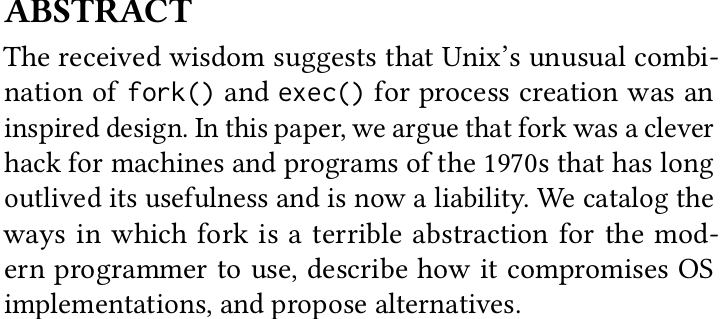
\includegraphics[width=5in]{../unix-api/fork-in-road-abs}
\end{frame}


\subsection{wait}

\againframe<5>{posixProcessFunctions}

\begin{frame}{wait/waitpid}
\begin{itemize}
\item \texttt{pid\_t waitpid(pid\_t pid, int *status, \\
              \hspace{5cm} int options)}
\item wait for a child process (with pid=\texttt{pid}) to finish
\item sets \texttt{*status} to its ``status information''
\vspace{.5cm}
\item \texttt{pid=-1} $\rightarrow$ wait for any child process instead
    \begin{itemize}
    \item \texttt{pid=0} almost the same
    \end{itemize}
\item options? see manual page (command \texttt{man waitpid})
    \begin{itemize}
        \item \texttt{0} --- no options
        %\item \myemph<2>{\texttt{WNOHANG}} --- return 0 rather than hanging if process not yet done
    \end{itemize}
\end{itemize}
\end{frame}

\begin{frame}[fragile,label=waitpidExample]{waitpid example}
\begin{lstlisting}[
    language=C++,
    style=smaller
]
#include <sys/wait.h>
...
  child_pid = fork();
  if (child_pid > 0) {
      /* Parent process */
      int status;
      waitpid(child_pid, &status, 0);
  } else if (child_pid == 0) {
      /* Child process */
      ...
\end{lstlisting}
\end{frame}



\subsection{summary diagram}

\usetikzlibrary{arrows.meta,decorations.pathmorphing,fadings}

\begin{frame}[fragile,label=typicalPatternSnake]{typical pattern}
\begin{tikzpicture}
\tikzset{
    thread/.style={very thick,draw,decorate,decoration=snake},
    split/.style={very thick,draw},
    marker/.style={thin,draw},
}
\path[thread] (0, 0) --  (0, -.5);
\node[anchor=south] at (0,0) {parent};
\node[anchor=north] (fork mark) at (0, -.5) {fork};
\draw[thread] (fork mark.south) -- (0, -2) node[below] (wait start) {waitpid};
\node (child start) at (9, -1.5) {child process};
\path[split] (fork mark) --  (child start);
\path[thread] (child start.south) -- (9, -2.5) node[below] (exec) {exec};
\path[thread] (exec.south) -- ++(0, -2) coordinate (exec done);
\path[marker] (exec done) -- ++(.5, 0) node[right] {exit()};
\path[split,dotted] (exec done) -- (0, -6);
\draw[very thick,dashed] (wait start) -- (0, -6);
\path[thread] (0, -6) -- ++(0, -3);
\end{tikzpicture}
\end{frame}


\begin{frame}[fragile,label=typicalPatternSnakeAlt]{typical pattern (alt)}
\begin{tikzpicture}
\tikzset{
    thread/.style={very thick,draw,decorate,decoration=snake},
    split/.style={very thick,draw},
    marker/.style={thin,draw},
}
\path[thread] (0, 0) --  (0, -.5);
\node[anchor=south] at (0,0) {parent};
\node[anchor=north] (fork mark) at (0, -.5) {fork};
\draw[thread] (fork mark.south) -- (0, -5.5) node[below] (wait start) {waitpid};
\node (child start) at (9, -1.5) {child process};
\path[split] (fork mark) --  (child start);
\path[thread] (child start.south) -- (9, -2.5) node[below] (exec) {exec};
\path[thread] (exec.south) -- ++(0, -1) coordinate (exec done);
\path[marker] (exec done) -- ++(.5, 0) node[right] {exit()};
\path[split,dotted] (exec done) -- (wait start.east);
%\draw[very thick,dashed] (wait start) -- (0, -6);
\path[thread] (wait start.south) -- ++(0, -3);
\end{tikzpicture}
\end{frame}

\begin{frame}[fragile,label=typicalPattern]{typical pattern (detail)}
\newcommand{\maincode}{
            pid = fork(); \\
            if (pid == 0) \{ \\
            \hspace{.5cm} exec\ldots(\ldots); \\
            \hspace{.5cm} \ldots \\
            \} else if (pid > 0) \{ \\
            \hspace{.5cm} waitpid(pid,\ldots); \\
            \hspace{.5cm} \ldots \\
            \} \\
            \ldots
}
\newcommand{\maincodeExec}{
            pid = fork(); \\
            if (pid == 0) \{ \\
            \hspace{.5cm} \myemph{exec\ldots(\ldots);} \\
            \hspace{.5cm} \ldots \\
            \} else if (pid > 0) \{ \\
            \hspace{.5cm} waitpid(pid,\ldots); \\
            \hspace{.5cm} \ldots \\
            \} \\
            \ldots
}
\newcommand{\maincodeWait}{
            pid = fork(); \\
            if (pid == 0) \{ \\
            \hspace{.5cm} exec\ldots(\ldots); \\
            \hspace{.5cm} \ldots \\
            \} else if (pid > 0) \{ \\
            \hspace{.5cm} \myemph{waitpid(pid,\ldots);} \\
            \hspace{.5cm} \ldots \\
            \} \\
            \ldots
}
\newcommand{\altcode}{
            main() \{ \\
            \hspace{.5cm} \ldots \\
            \} \\
}
\begin{tikzpicture}
\tikzset{
    code box/.style={draw,thick,font=\tt\fontsize{9}{10}\selectfont,align=left},
    with the code/.style={
        code box,
    },
    with the other code/.style={
        code box,
    }
}
\node[with the code] (start) {\maincode};
\node[with the code,anchor=north west] (parent first) at ([xshift=2cm,yshift=1cm]start.south east) {\maincodeWait};
\node[with the code,anchor=south west] (child first) at ([xshift=2cm,yshift=-1cm]start.north east) {\maincodeExec};
\node[with the other code,anchor=north west] (child second) at ([xshift=2cm]child first.north east) {\altcode};

\begin{scope}[very thick,>=Latex]
\draw[->] (start) -- (parent first);
\draw[->] (start) -- (child first);
\draw[->] (child first) -- (child second);
\end{scope}
\end{tikzpicture}
\end{frame}



\subsection{waiting for more than one?}


\usetikzlibrary{arrows.meta,decorations.pathmorphing,fadings}

\begin{frame}[fragile,label=patternMultSnake]{pattern with multiple?}
\begin{tikzpicture}
\tikzset{
    thread/.style={very thick,draw,decorate,decoration=snake},
    split/.style={very thick,draw},
    marker/.style={thin,draw},
}
\path[thread] (0, 0) --  (0, -.5);
\node[anchor=south] at (0,0) {parent};
\node[anchor=north] (fork mark 1) at (0, -.5) {fork};
\draw[thread] (fork mark 1) -- ++(0, -1) node[below] (fork mark 2) {fork};
\draw[thread] (fork mark 2.south) -- ++(0, -1) node[below] (wait 1 start) {waitpid(first,\ldots)};
\node (child 1 start) at (9, -1.5) {first child process};
\node (child 2 start) at (4, -2.5) {second child process};
\path[split] (fork mark 1) --  (child 1 start);
\path[split] (fork mark 2) --  (child 2 start);
\path[thread] (child 1 start.south) -- ++(0, -1) node[below] (exec 1) {exec};
\path[thread] (exec 1.south) -- ++(0, -2) coordinate (exec 1 done);
\path[marker] (exec 1 done) -- ++(.5, 0) node[right] {exit()};
\path[thread] (child 2 start.south) -- ++(0, -1) node[below] (exec 2) {exec};
\path[thread] (exec 2.south) -- ++ (0, -0.5) coordinate (exec 2 done);
\path[marker] (exec 2 done) -- ++(.5, 0) node[right] {exit()};
\path[split,dotted] (exec 1 done) -- (0, -6) coordinate (wait 1 done);;
\draw[very thick,dashed] (wait 1 start) -- (wait 1 done);
\draw[thread] (wait 1 done) -- ++(0, -.5) node[below] (wait 2 start) { waitpid(second,\ldots) };
\path[split,dotted] (exec 2 done) -- (wait 2 start);
\draw[overlay,thread] (wait 2 start.south) -- ++ (0, -2);
\end{tikzpicture}
\end{frame}


\againframe<6>{posixProcessFunctions}

\subsection{exercises (fork+exec+wait)}

\begin{frame}[fragile,label=fork-wait-ex1]{exercise (1)}
\vspace{-.25cm}
\begin{lstlisting}[basicstyle=\fontsize{9.5}{10.5}\tt\selectfont]
int main() {
    pid_t pids[2]; const char *args[] = {"echo", "ARG", NULL};
    const char *extra[] = {"L1", "L2"};
    for (int i = 0; i < 2; ++i) {
        pids[i] = fork();
        if (pids[i] == 0) {
            args[1] = extra[i];
            execv("/bin/echo", args);
        }
    }
    for (int i = 0; i < 2; ++i) {
        waitpid(pids[i], NULL, 0);
    }
}
\end{lstlisting}
\newcommand{\shownewline}{ {\fontsize{9}{10}\selectfont(newline)} }
Assuming fork and execv do not fail, which are possible outputs?
\begin{tabular}{llll}
\bfseries A. & \tt L1\shownewline L2 & \bfseries D. & A and B \\
\bfseries B. & \tt L1\shownewline L2\shownewline L2 & \bfseries E. & A and C \\
\bfseries C. & \tt L2\shownewline L1 & \bfseries F. & all of the above \\
    ~ &  ~ & \bfseries G. & something else \\
\end{tabular}
\end{frame}

\iftoggle{heldback}{\providecommand{\correct}[1]{#1}}{\providecommand{\correct}[1]{\myemph<2>{#1}}}

\begin{frame}[fragile,label=fork-wait-ex2]{exercise (2)}
\vspace{-.4cm}
\begin{lstlisting}[basicstyle=\fontsize{9.5}{10.5}\tt\selectfont]
int main() {
    pid_t pids[2]; const char *args[] = {"echo", "0", NULL};
    for (int i = 0; i < 2; ++i) {
        pids[i] = fork();
        if (pids[i] == 0) { execv("/bin/echo", args); }
    }
    printf("1\n"); fflush(stdout);
    for (int i = 0; i < 2; ++i) {
        waitpid(pids[i], NULL, 0);
    }
    printf("2\n"); fflush(stdout);
}
\end{lstlisting}
\newcommand{\shownewline}{ {\normalfont\fontsize{9}{10}\selectfont(newline)} }
Assuming fork and execv do not fail, which are possible outputs?
\begin{tabular}{llll}
\bfseries A. & \tt 0\shownewline 0\shownewline 1\shownewline 2 & \bfseries E. & \correct{A, B, and C} \\
\bfseries B. & \tt 0\shownewline 1\shownewline 0\shownewline 2 & \bfseries F. & C and D \\
\bfseries C. & \tt 1\shownewline 0\shownewline 0\shownewline 2 & \bfseries G. & all of the above \\
\bfseries D. & \tt 1\shownewline 0\shownewline 2\shownewline 0 & \bfseries H. & something else \\
\end{tabular}
\end{frame}




\section{shells}

\subsection{shells, the concept}

\begin{frame}{shell}
\begin{itemize}
    \item allow user (= person at keyboard) to run applications
    \item user's wrapper around process-management functions
\end{itemize}
\end{frame}

\begin{frame}{aside: shell forms}
\begin{itemize}
    \item POSIX: command line you have used before
        \vspace{.5cm}
    \item also: graphical shells
        \begin{itemize}
        \item e.g. OS X Finder, Windows explorer
        \end{itemize}
    \item other types of command lines?
    \item completely different interfaces?
\end{itemize}
\end{frame}



\subsection{I/O redirection: syntax, method preview}

\againframe<4>{commandLineFeatures}

\subsection{pipelines}

\againframe<5>{commandLineFeatures}

\section{files in POSIX, part 1}

\subsection{interlude: file descriptors}

\begin{frame}[fragile,label=fds]{file descriptors}
\begin{lstlisting}[language=C,style=smaller]
struct process_info {  /* <-- in the kernel somewhere */
    ...
    struct open_file_description *files[SIZE];
    ...
};
...
process->files[file_descriptor]
\end{lstlisting}
    \begin{itemize}
    \item Unix: every process has \\
        array (or similar) of \textit{open file descriptions}
    \item ``open file'': {\small terminal $\cdot$ socket $\cdot$ regular file $\cdot$ pipe}
    \item file descriptor = index into array
        \begin{itemize}
        \item usually what's used with system calls
        \item stdio.h FILE*s usually have file descriptor + buffer
        \end{itemize}
    \end{itemize}
\end{frame}






\begin{frame}{special file descriptors}
\begin{itemize}
\item file descriptor 0 = standard input
\item file descriptor 1 = standard output
\item file descriptor 2 = standard error
\vspace{.5cm}
\item constants in \texttt{unistd.h}
    \begin{itemize} \item \texttt{STDIN\_FILENO}, \texttt{STDOUT\_FILENO}, \texttt{STDERR\_FILENO} \end{itemize}
\vspace{.5cm}
\item<2-> but you can't choose which number \texttt{open} assigns\ldots?
    \begin{itemize}
    \item more on this later
    \end{itemize}
\end{itemize}
\end{frame}



\subsection{getting file descriptors}


\begin{frame}[fragile,label=gettingFds]{getting file descriptors}
\begin{lstlisting}[
    language=C++,
    moredelim={**[is][\btHL<1-|handout:1->]{@1}{1@}},
    style=smaller
]
int read_fd = open("dir/file1", O_RDONLY);
int write_fd = open("/other/file2", O_WRONLY | ...);
int rdwr_fd = open("file3", O_RDWR);
\end{lstlisting}
\begin{itemize}
\item used internally by fopen(), etc.
\item also for files without normal filenames\ldots:
\end{itemize}
\begin{lstlisting}[
    language=C++,
    moredelim={**[is][\btHL<1-|handout:1->]{@1}{1@}},
    style=smaller,
]
int fd = shm_open("/shared_memory", O_RDWR, 0666); // shared memory
int socket_fd = socket(AF_INET, SOCK_STREAM, 0); // TCP socket
int term_fd = posix_openpt(O_RDWR); // pseudo-terminal
int pipe_fds[2]; pipe(pipefds); // "pipes" (later)
...
\end{lstlisting}
\end{frame}


\subsection{close}

\begin{frame}[fragile,label=close]{close}
\begin{lstlisting}[language=C++]
int close(int fd);
\end{lstlisting}
\begin{itemize}
\item close the file descriptor, deallocating that array index
    \begin{itemize}
    \item does not affect other file descriptors \\ that refer to same ``open file description''
    \item (e.g. in \texttt{fork()}ed child or created via (later) \texttt{dup2})
    \end{itemize}
\item if last file descriptor for open file description, resources deallocated
\vspace{.5cm}
\item returns 0 on success
\item returns -1 on error
    \begin{itemize}
    \item e.g. ran out of disk space while finishing saving file
    \end{itemize}
\end{itemize}
\end{frame}


\subsection{Shell: redirection}

\usetikzlibrary{matrix,patterns,arrows.meta,decorations.pathreplacing,shapes.misc,fit}

\begin{frame}[fragile,label=redirectExample]{shell redirection}
\begin{itemize}
\item \verb|./my_program ... < input.txt|:
    \begin{itemize}
    \item run \verb|./my_program ...| but use \verb|input.txt| as input
    \item like we copied and pasted the file into the terminal
    \end{itemize}
\vspace{.5cm}
\item \verb|echo foo > output.txt|:
    \begin{itemize}
    \item runs \verb|echo foo|, sends output to \verb|output.txt|
    \item like we copied and pasted the output into that file
    \item (as it was written)
    \end{itemize}
\end{itemize}
\end{frame}

\begin{frame}[fragile,label=forkTrick]{fork copies open file list}
\begin{tikzpicture}
\tikzset{
    >=Latex,
    pcb/.style={
        tight matrix,
        column 1/.style={nodes={draw,thin,text width=2.5cm,font=\small,minimum height=0.45cm}},
        column 2/.style={nodes={draw,thin,text width=4.75cm,font=\fontsize{9}{10}\tt\selectfont,minimum height=0.45cm}},
    },
    page/.style={
        draw,thick,
        pattern=north west lines,
        minimum width=2cm,
        node contents={~},
    },
    pointer/.style={
        draw,very thick,-Latex,
    },
    pointer light/.style={
        draw,thick,-Latex,
    },
    tall/.style={
        minimum height=0.85cm
    },
    taller/.style={
        minimum height=1.2cm
    },
    one pt/.style={
        fill=blue!40,
    },
    one pt line/.style={
        draw=blue!80!black,
        alt=<2->{opacity=0.0},
    },
    one memory/.style={
        fill=green!40,
    },
    one memory line/.style={
        draw=green!80!black,
        alt=<2->{opacity=0.0},
    },
    two pt/.style={
        fill=orange!40,
    },
    two pt line/.style={
        draw=orange!80!black,
        alt=<2->{opacity=0.0},
    },
    two memory/.style={
        fill=violet!40,
    },
    two memory line/.style={
        draw=violet!80!black,
        alt=<2->{opacity=0.0},
    },
    fork line/.style={
        draw=black!30,line width=2mm,-{Latex[length=6mm]}
    },
    marked/.style={draw=red,ultra thick},
}
\matrix[pcb,label={[font=\small]north:parent process control block}] (proc one) {
    |[tall]| user regs \&
    |[tall]|
    {eax=\sout<1->{42}\only<1->{\textit{\myemph<0>{child (new) pid}}}, \\ ecx=133,} \ldots \\
    page table \& |[one pt]| ~ \\
    |[taller]| open files \& |[taller,marked,alias=old files]| {fd 0: \ldots \\ fd 1: \ldots \\ \ldots } \\
    \ldots \& \ldots \\
};
\newcommand{\halfvthick}{.2mm}
\node[draw,very thick,pattern=north west lines,minimum width=1.5cm,minimum height=3cm,anchor=north west,
    label={north:memory}] (memory) at ([xshift=3cm,yshift=0cm]proc one.north east) {};
\draw[pointer,one pt line] (proc one-2-2.east) -- ++(1cm,0cm) |- ([yshift=-1.3cm]memory.north west);
\foreach \y in {-1.3cm} {
    \draw[very thick,one pt] ([yshift=\y,xshift=\halfvthick]memory.north west) rectangle ++ (1.5cm,-1mm);
}
\coordinate (one pt loc) at ([yshift=-1.35cm,xshift=\halfvthick]memory.north west);
\draw[pointer light,one memory line] ([yshift=-.1mm]one pt loc) -- ++(-.25cm,0cm) |- ([yshift=-0.1cm]memory.north west);
\draw[pointer light,one memory line] ([yshift=-.2mm]one pt loc) -- ++(-.35cm,0cm) |- ([yshift=-0.6cm]memory.north west);
\draw[pointer light,one memory line] ([yshift=.3mm]one pt loc) -- ++(-.45cm,0cm) |- ([yshift=-0.7cm]memory.north west);
\foreach \y in {-0.5cm,-0.7cm,-0.8mm} {
    \draw[very thick,one memory] ([yshift=\y,xshift=\halfvthick]memory.north west) rectangle ++ (1.5cm,-1mm);
}
\matrix[pcb,anchor=north west,label={[font=\small]north:child process control block}] (proc two) at ([yshift=-1cm]proc one.south west) {
    |[tall]| user regs \&
    |[tall]|
    {eax=\sout<1->{42}\only<1->{\myemph<0>{0}}, \\ ecx=133, \ldots} \\
    pagetable \& |[two pt]| ~ \\
    |[taller]| open files \& |[taller,marked,alias=new files]| {fd 0: \ldots \\ fd 1: \ldots \\ \ldots } \\
    \ldots \& \ldots \\
};
\draw[fork line] ([xshift=-0.25cm]proc one.west) -- ++(-1cm,0cm) |- ([xshift=-0.25cm]proc two.west)
    node[pos=0.25,right] {copy};
\draw[pointer,two pt line] (proc two-2-2.east) -- ++(1cm,0cm) |- ([yshift=-2.3cm]memory.north west);
\foreach \y in {-2.3cm} {
    \draw[very thick,two pt] ([yshift=\y,xshift=\halfvthick]memory.north west) rectangle ++ (1.5cm,-1mm);
}
\coordinate (two pt loc) at ([yshift=-2.35cm,xshift=\halfvthick]memory.north west);
\draw[pointer light,two memory line] ([yshift=-.1mm]two pt loc) -- ++(-.75cm,0cm) |- ([yshift=-2.4cm]memory.north west);
\draw[pointer light,two memory line] ([yshift=-.2mm]two pt loc) -- ++(-.85cm,0cm) |- ([yshift=-2.6cm]memory.north west);
\draw[pointer light,two memory line] ([yshift=-.3mm]two pt loc) -- ++(-.95cm,0cm) |- ([yshift=-2.7cm]memory.north west);
\foreach \y in {-2.4cm,-2.6cm,-2.7cm} {
    \draw[very thick,two memory] ([yshift=\y,xshift=\halfvthick]memory.north west) rectangle ++ (1.5cm,-1mm);
}
\draw[fork line] ([yshift=-0.9cm,xshift=.5cm]memory.north east) coordinate (one memory)-- ++(1.2cm, 0cm) |- ([yshift=-2.6cm,xshift=.5cm]memory.north east) coordinate (two memory)
    node[pos=0.25,left] {copy};
\draw[ultra thick,decorate,decoration={brace,mirror}] ([xshift=-.25cm,yshift=-8mm]one memory) -- ([xshift=-.25cm,yshift=8mm]one memory);
\draw[ultra thick,decorate,decoration={brace,mirror}] ([xshift=-.25cm,yshift=-4mm]two memory) -- ([xshift=-.25cm,yshift=4mm]two memory);
\begin{visibleenv}<2->
\node[draw, very thick,anchor=north west,font=\small,align=left] (fd0) at ([yshift=-1cm,xshift=-2.5cm]memory.south) {
    open file description (stdin)
};
\node[draw, very thick,anchor=north west,font=\small,align=left] (fd1) at ([yshift=-1mm]fd0.south west) {
    open file description (stdout)
};
\draw[violet,->,ultra thick] ([xshift=1.5cm,yshift=-.25cm]old files.north west) -| ([xshift=-1cm]fd0.west) -- (fd0.west);
\draw[violet,->,ultra thick] ([xshift=1.5cm,yshift=-.25cm]new files.north west) -| ([xshift=-1cm]fd0.west) -- (fd0.west);
\draw[blue,->,ultra thick] ([xshift=1.5cm,yshift=-.55cm]old files.north west) -| ([xshift=-.75cm]fd1.west) -- (fd1.west);
\end{visibleenv}
\begin{visibleenv}<2>
\draw[blue,->,ultra thick] ([xshift=1.5cm,yshift=-.55cm]new files.north west) -| ([xshift=-.75cm]fd1.west) -- (fd1.west);
\end{visibleenv}
\begin{visibleenv}<3->
    \draw[blue,->,opacity=0.5,ultra thick] ([xshift=1.5cm,yshift=-.55cm]new files.north west) -| ([xshift=-.75cm]fd1.west) -- (fd1.west);
\node[draw,dotted,red,fill=red!5,ultra thick,anchor=north west,font=\small,align=left] (fd2) at ([yshift=-1mm]fd1.south west) {
    redirected-to stdout? \\
    (set after fork, before exec)
};
\draw[red,dotted,->,line width=1.2mm] ([xshift=1.5cm,yshift=-.55cm]new files.north west) -| ([xshift=-.75cm]fd2.west) -- (fd2.west);
\end{visibleenv}
\end{tikzpicture}
\end{frame}

\begin{frame}[fragile,label=typicalPatternRedirect]{typical pattern with redirection}
\newcommand{\maincode}{
            pid = fork(); \\
            if (pid == 0) \{ \\
            \hspace{.5cm} open new files; \\
            \hspace{.5cm} exec\ldots(\ldots); \\
            \hspace{.5cm} \ldots \\
            \} else if (pid > 0) \{ \\
            \hspace{.5cm} waitpid(pid,\ldots); \\
            \hspace{.5cm} \ldots \\
            \} \\
            \ldots
        }
\newcommand{\maincodeWait}{
            pid = fork(); \\
            if (pid == 0) \{ \\
            \hspace{.5cm} open new files; \\
            \hspace{.5cm} exec\ldots(\ldots); \\
            \hspace{.5cm} \ldots \\
            \} else if (pid > 0) \{ \\
            \hspace{.5cm} \myemph{waitpid(pid,\ldots)}; \\
            \hspace{.5cm} \ldots \\
            \} \\
            \ldots
        }
\newcommand{\maincodeFork}{
            pid = \myemph{fork()}; \\
            if (pid == 0) \{ \\
            \hspace{.5cm} open new files; \\
            \hspace{.5cm} exec\ldots(\ldots); \\
            \hspace{.5cm} \ldots \\
            \} else if (pid > 0) \{ \\
            \hspace{.5cm} waitpid(pid,\ldots); \\
            \hspace{.5cm} \ldots \\
            \} \\
            \ldots
        }
\newcommand{\maincodeOpenNew}{
            pid = fork(); \\
            if (pid == 0) \{ \\
            \hspace{.5cm} \myemph{open new files}; \\
            \hspace{.5cm} exec\ldots(\ldots); \\
            \hspace{.5cm} \ldots \\
            \} else if (pid > 0) \{ \\
            \hspace{.5cm} waitpid(pid,\ldots); \\
            \hspace{.5cm} \ldots \\
            \} \\
            \ldots
}
\newcommand{\altcode}{
            main() \{ \\
            \hspace{.5cm} \ldots \\
            \}
}
\begin{tikzpicture}
\tikzset{
    code box/.style={draw,thick,font=\tt\fontsize{9}{10}\selectfont,align=left},
    with the code/.style={
        code box,
    },
    with the other code/.style={
        code box,
    }
}
\node[with the code] (start) {\maincodeFork};
\node[with the code,anchor=south west,
      label={[font=\small,label distance=-1mm,overlay]north:parent}] (parent first) at ([xshift=4cm,yshift=-1.5cm]start.north east) {\maincodeWait};
\node[with the code,anchor=north west,
      label={[font=\small,label distance=-1mm]north:child}] (child first) at ([xshift=1.25cm,yshift=2cm]start.south east) {\maincodeOpenNew};
\node[with the other code,anchor=north west] (child second) at ([xshift=2cm]child first.north east) {\altcode};

\begin{scope}[very thick,>=Latex]
\draw[->] ([yshift=1.25cm]start.east) -- (parent first);
\draw[->] ([yshift=-1.25cm]start.east) -- (child first);
\draw[->] (child first) -- (child second);
\end{scope}
\end{tikzpicture}
\end{frame}

\begin{frame}{redirecting with exec}
\begin{itemize}
\item standard output/error/input are files
    \begin{itemize}
    \item (C stdout/stderr/stdin; C++ cout/cerr/cin)
    \end{itemize}
\vspace{.5cm}
\item (probably after forking) open files to redirect
\item \ldots and make them be standard output/error/input
    \begin{itemize}
    \item using \texttt{dup2()} library call
    \end{itemize}
\item then exec, preserving new standard output/etc.
\end{itemize}
\end{frame}


\subsection{dup2: redirection mechanism}

\begin{frame}<1>[fragile,label=reassign]{reassigning file descriptors}
\begin{itemize}
\item redirection: \verb|./program >output.txt|
\item step 1: open output.txt for writing, get new file descriptor
\item step 2: \myemph<2>{make that new file descriptor stdout (number 1)}
\vspace{.5cm}
\item<2-> tool: \texttt{int dup2(int oldfd, int newfd)} \\
        make \texttt{newfd} refer to same open file as \texttt{oldfd}
    \begin{itemize}
    \item same \textit{open file description}
    \item shares the current location in the file
    \item (even after more reads/writes)
    \end{itemize}
\item<2-> what if newfd already allocated --- closed, then reused
\end{itemize}
\end{frame}

\begin{frame}[fragile,label=dup2AndTable]{reassigning and file table}
\begin{lstlisting}[language=C,style=smaller]
// something like this in OS code
struct process_info { 
    ...
    struct open_file_description *files[SIZE];
    ....
};
...
process->files[STDOUT_FILENO] = process->files[opened-fd];
\end{lstlisting}
\begin{itemize}
\item syscall: \texttt{dup2(\textit{opened-fd}, STDOUT\_FILENO);}
\end{itemize}
\end{frame}

\againframe<2>{reassign}

\begin{frame}[fragile,label=dup2example]{dup2 example}
redirects stdout to output to \texttt{output.txt}:
\begin{lstlisting}[language=C++,style=small]
fflush(stdout);  /* clear printf's buffer */
int fd = open("output.txt",
              O_WRONLY | O_CREAT | O_TRUNC);
if (fd < 0)
    do_something_about_error();

dup2(fd, STDOUT_FILENO);
/* now both write(fd, ...) and write(STDOUT_FILENO, ...) 
   write to output.txt
   */

close(fd); /* only close original, copy still works! */

printf("This will be sent to output.txt.\n");
\end{lstlisting}
\end{frame}


\subsection{open/close/dup/fork and fd array}

\begin{frame}[fragile,label=openCloseAndFdArray]{open/dup/close/etc. and fd array}
\begin{lstlisting}[
    language=C++,
    moredelim={**[is][\btHL<1-|handout:1->]{@1}{1@}},
    style=smaller
]
// something like this in OS code
struct process_info {
  ...
  @1struct open_file_description *files[NUM];1@  
};
\end{lstlisting}
\begin{itemize}
\item open: \lstinline|files[new_fd] = ...;|
\item dup2(from, to): \lstinline|files[to] = files[from];|
\item close: \lstinline|files[fd] = NULL;|
\item fork: 
\begin{lstlisting}
  for (int i = ...)
      child->files[i] = parent->files[i];
\end{lstlisting}
\vspace{.25cm}
\item (plus extra work to avoid leaking memory)
\end{itemize}
\end{frame}


\subsection{exercise (read/write/dup2)}

\begin{frame}[fragile,label=ex]{exercise}
\begin{lstlisting}[style=small]
int fd = open("output.txt", O_WRONLY|O_CREAT|O_TRUNC, 0666);
write(fd, "A", 1);
dup2(STDOUT_FILENO, 100);
dup2(fd, STDOUT_FILENO);
write(STDOUT_FILENO, "B", 1);
write(fd, "C", 1);
close(fd);
write(STDOUT_FILENO, "D", 1);
write(100, "E", 1);
\end{lstlisting}
\small Assume \texttt{open()} and \texttt{dup2()} \textit{do not fail},
\texttt{write()} does not fail as long as the fd it writes to is open,
fd \texttt{100} was closed and is not what open returns, and \texttt{STDOUT\_FILENO} is initially open.
What is written to \texttt{output.txt}? \\
\begin{tabular}{llllll}
\textbf{A.} & ABCDE & \textbf{C.} & ABC & \textbf{E.} something else \\
\textbf{B.} & ABCD & \textbf{D.} & ACD \\
\end{tabular}
\end{frame}


\section{pipelines}

\subsection{pipe}

\begin{frame}{pipes}
\begin{itemize}
\item special kind of file: pipes
\item bytes go in one end, come out the other --- once
\vspace{.5cm}
\item created with \texttt{pipe()} library call
\item intended use: communicate between processes
    \begin{itemize}
    \item like implementing shell pipelines
    \end{itemize}
\end{itemize}
\end{frame}

\begin{frame}[fragile,label=pipe]{pipe()}
\begin{lstlisting}[language=C++,style=small]
int pipe_fd[2];
if (pipe(pipe_fd) < 0)
    handle_error();
/* normal case: */
int read_fd = pipe_fd[0];
int write_fd = pipe_fd[1];
\end{lstlisting}
then from one process\ldots
\begin{lstlisting}[language=C++,style=small]
write(write_fd, ...);
\end{lstlisting}
and from another
\begin{lstlisting}[language=C++,style=small]
read(read_fd, ...);
\end{lstlisting}
\end{frame}

\begin{frame}[fragile,label=pipeAndBlocking]{pipe() and blocking}
\myemph{BROKEN} example:
\begin{lstlisting}[language=C++,style=small]
int pipe_fd[2];
if (pipe(pipe_fd) < 0)
    handle_error();
int read_fd = pipe_fd[0];
int write_fd = pipe_fd[1];
write(write_fd, some_buffer, some_big_size);
read(read_fd, some_buffer, some_big_size);
\end{lstlisting}
This is likely to \myemph{not terminate}. What's the problem?
\end{frame}

\begin{frame}[fragile,label=pipeExample]{pipe example (1)}
\begin{lstlisting}[
    language=C++,
    style=smaller,
    moredelim={**[is][\btHL<2|handout:0>]{@2}{2@}},
    moredelim={**[is][\btHL<3|handout:2>]{@3}{3@}},
    moredelim={**[is][\btHL<4|handout:3>]{@4}{4@}},
]
int pipe_fd[2];
if (pipe(pipe_fd) < 0)
    handle_error(); /* e.g. out of file descriptors */
int read_fd = pipe_fd[0];
int write_fd = pipe_fd[1];
@2child_pid = fork();2@
@2if (child_pid  == 0) {2@
    /* in child process, write to pipe */
    @4close(read_fd);4@
    write_to_pipe(write_fd); /* function not shown */
    exit(EXIT_SUCCESS);
@2} else if (child_pid > 0) {2@
    /* in parent process, read from pipe */
    @3close(write_fd);3@
    read_from_pipe(read_fd); /* function not shown */
    @2waitpid(child_pid, NULL, 0);2@
    @4close(read_fd);4@
} @2else {2@ /* fork error */ }
\end{lstlisting}
\begin{tikzpicture}[overlay,remember picture]
\coordinate (box place) at ([xshift=-1cm,yshift=-1cm]current page.north east);
\tikzset{
    box/.style={draw=red,thick,fill=white,anchor=north east,at={(box place)},align=left,font=\small},
}
\begin{visibleenv}<2|handout:0>
\node[box] {
    `standard' pattern with fork()
};
\end{visibleenv}
\begin{visibleenv}<3|handout:2>
\node[box] {
    read() will not indicate \\
    end-of-file if write fd is open  \\
    (any copy of it)
};
\end{visibleenv}
\begin{visibleenv}<4|handout:3>
\node[box] {
    have habit of closing \\
    to avoid `leaking' file descriptors \\
    you can run out
};
\end{visibleenv}
\end{tikzpicture}
\end{frame}


\subsection{pipe and pipelines}

\usetikzlibrary{decorations.pathmorphing}

\begin{frame}[fragile,label=pipeAndPipelines]{pipe and pipelines}
\begin{Verbatim}[frame=single,fontsize=\small]
ls -1 | grep foo
\end{Verbatim}
\begin{lstlisting}[language=C++,style=smaller]
pipe(pipe_fd);
ls_pid = fork();
if (ls_pid == 0) {
    dup2(pipe_fd[1], STDOUT_FILENO);
    close(pipe_fd[0]); close(pipe_fd[1]);
    char *argv[] = {"ls", "-1", NULL};
    execv("/bin/ls", argv);
}
grep_pid = fork();
if (grep_pid == 0) {
    dup2(pipe_fd[0], STDIN_FILENO);
    close(pipe_fd[0]); close(pipe_fd[1]);
    char *argv[] = {"grep", "foo", NULL};
    execv("/bin/grep", argv);
}
close(pipe_fd[0]); close(pipe_fd[1]);
/* wait for processes, etc. */
\end{lstlisting}
\end{frame}

\begin{frame}[fragile,label=pipeDiagram]{example execution}
\begin{tikzpicture}
\tikzset{
    thread/.style={very thick,draw,decorate,decoration=snake},
    split/.style={very thick,draw},
    marker/.style={thin,draw},
}
\path[thread] (0, 0) --  (0, -8);
    \node[anchor=south] at (0,0) {parent};
\path[marker] (0, -.5) -- ++(1, 0) node[right] {\texttt{pipe()} --- fds 3 [read], 4 [write]};
    \path[split] (0, -1) --  (9, -2) node[right] {child 1};
    \path[marker] (9, -3) -- ++(.5, 0) node[right] {4$\rightarrow$ stdout};
    \path[marker] (9, -4) -- ++(.5, 0) node[right] {close 3,4};
    \path[thread] (9, -2) -- (9, -5) node[below] (exec ls) {exec ls};
    \path[thread] (exec ls.south) -- ++(0, -.5cm);

    \path[split] (0, -2) --  (5, -3) node[right] {child 2};
    \path[marker] (5, -4) -- ++(.5, 0) node[right] {3$\rightarrow$ stdin};
    \path[marker] (5, -5) -- ++(.5, 0) node[right] {close 3,4};
    \path[thread] (5, -3) -- (5, -6) node[below] (exec grep) {exec grep};
    \path[thread] (exec grep.south) -- ++(0, -.5cm);
    \path[marker] (0, -5.5) -- ++(.5, 0) node[right] {close 3,4};
\end{tikzpicture}
\end{frame}


% FIXME: better understanding that this works without write()/read() specifically?



\section{POSIX api summary}
\begin{frame}{Unix API summary}
    \begin{itemize}
    \item spawn and wait for program: \texttt{fork} (copy), then
        \begin{itemize}
        \item in child: setup, then \texttt{execv}, etc. (replace copy)
        \item in parent: \texttt{waitpid}
        \end{itemize}
    \item files: open, read and/or write, close
        \begin{itemize}
        \item one interface for regular files, pipes, network, devices, \ldots
        \end{itemize}
    \item file descriptors are indices into per-process array
        \begin{itemize}
        \item index 0, 1, 2 = stdin, stdout, stderr
        \item \texttt{dup2} --- assign one index to another
        \item \texttt{close} --- deallocate index
        \end{itemize}
    \item redirection
        \begin{itemize}
        \item open() to create new file descriptors
        \item dup2 in child to assign file descriptor to index 0, 1
        \end{itemize}
    \end{itemize}
\end{frame}


\section{backup slides}
\begin{frame}{}
\end{frame}

\begin{frame}{backup slides}
\end{frame}

\subsection{POSIX and Unix}

\usetikzlibrary{calc}

\begin{frame}{this class: focus on Unix}
    \begin{itemize}
    \item Unix-like OSes will be our focus
    \item we have source code
    \item used to from 2150, etc.?
    \item have been around for a while
    \item xv6 imitates Unix
    \end{itemize}
\end{frame}

\begin{frame}{Unix history}
\vspace{-.5cm}
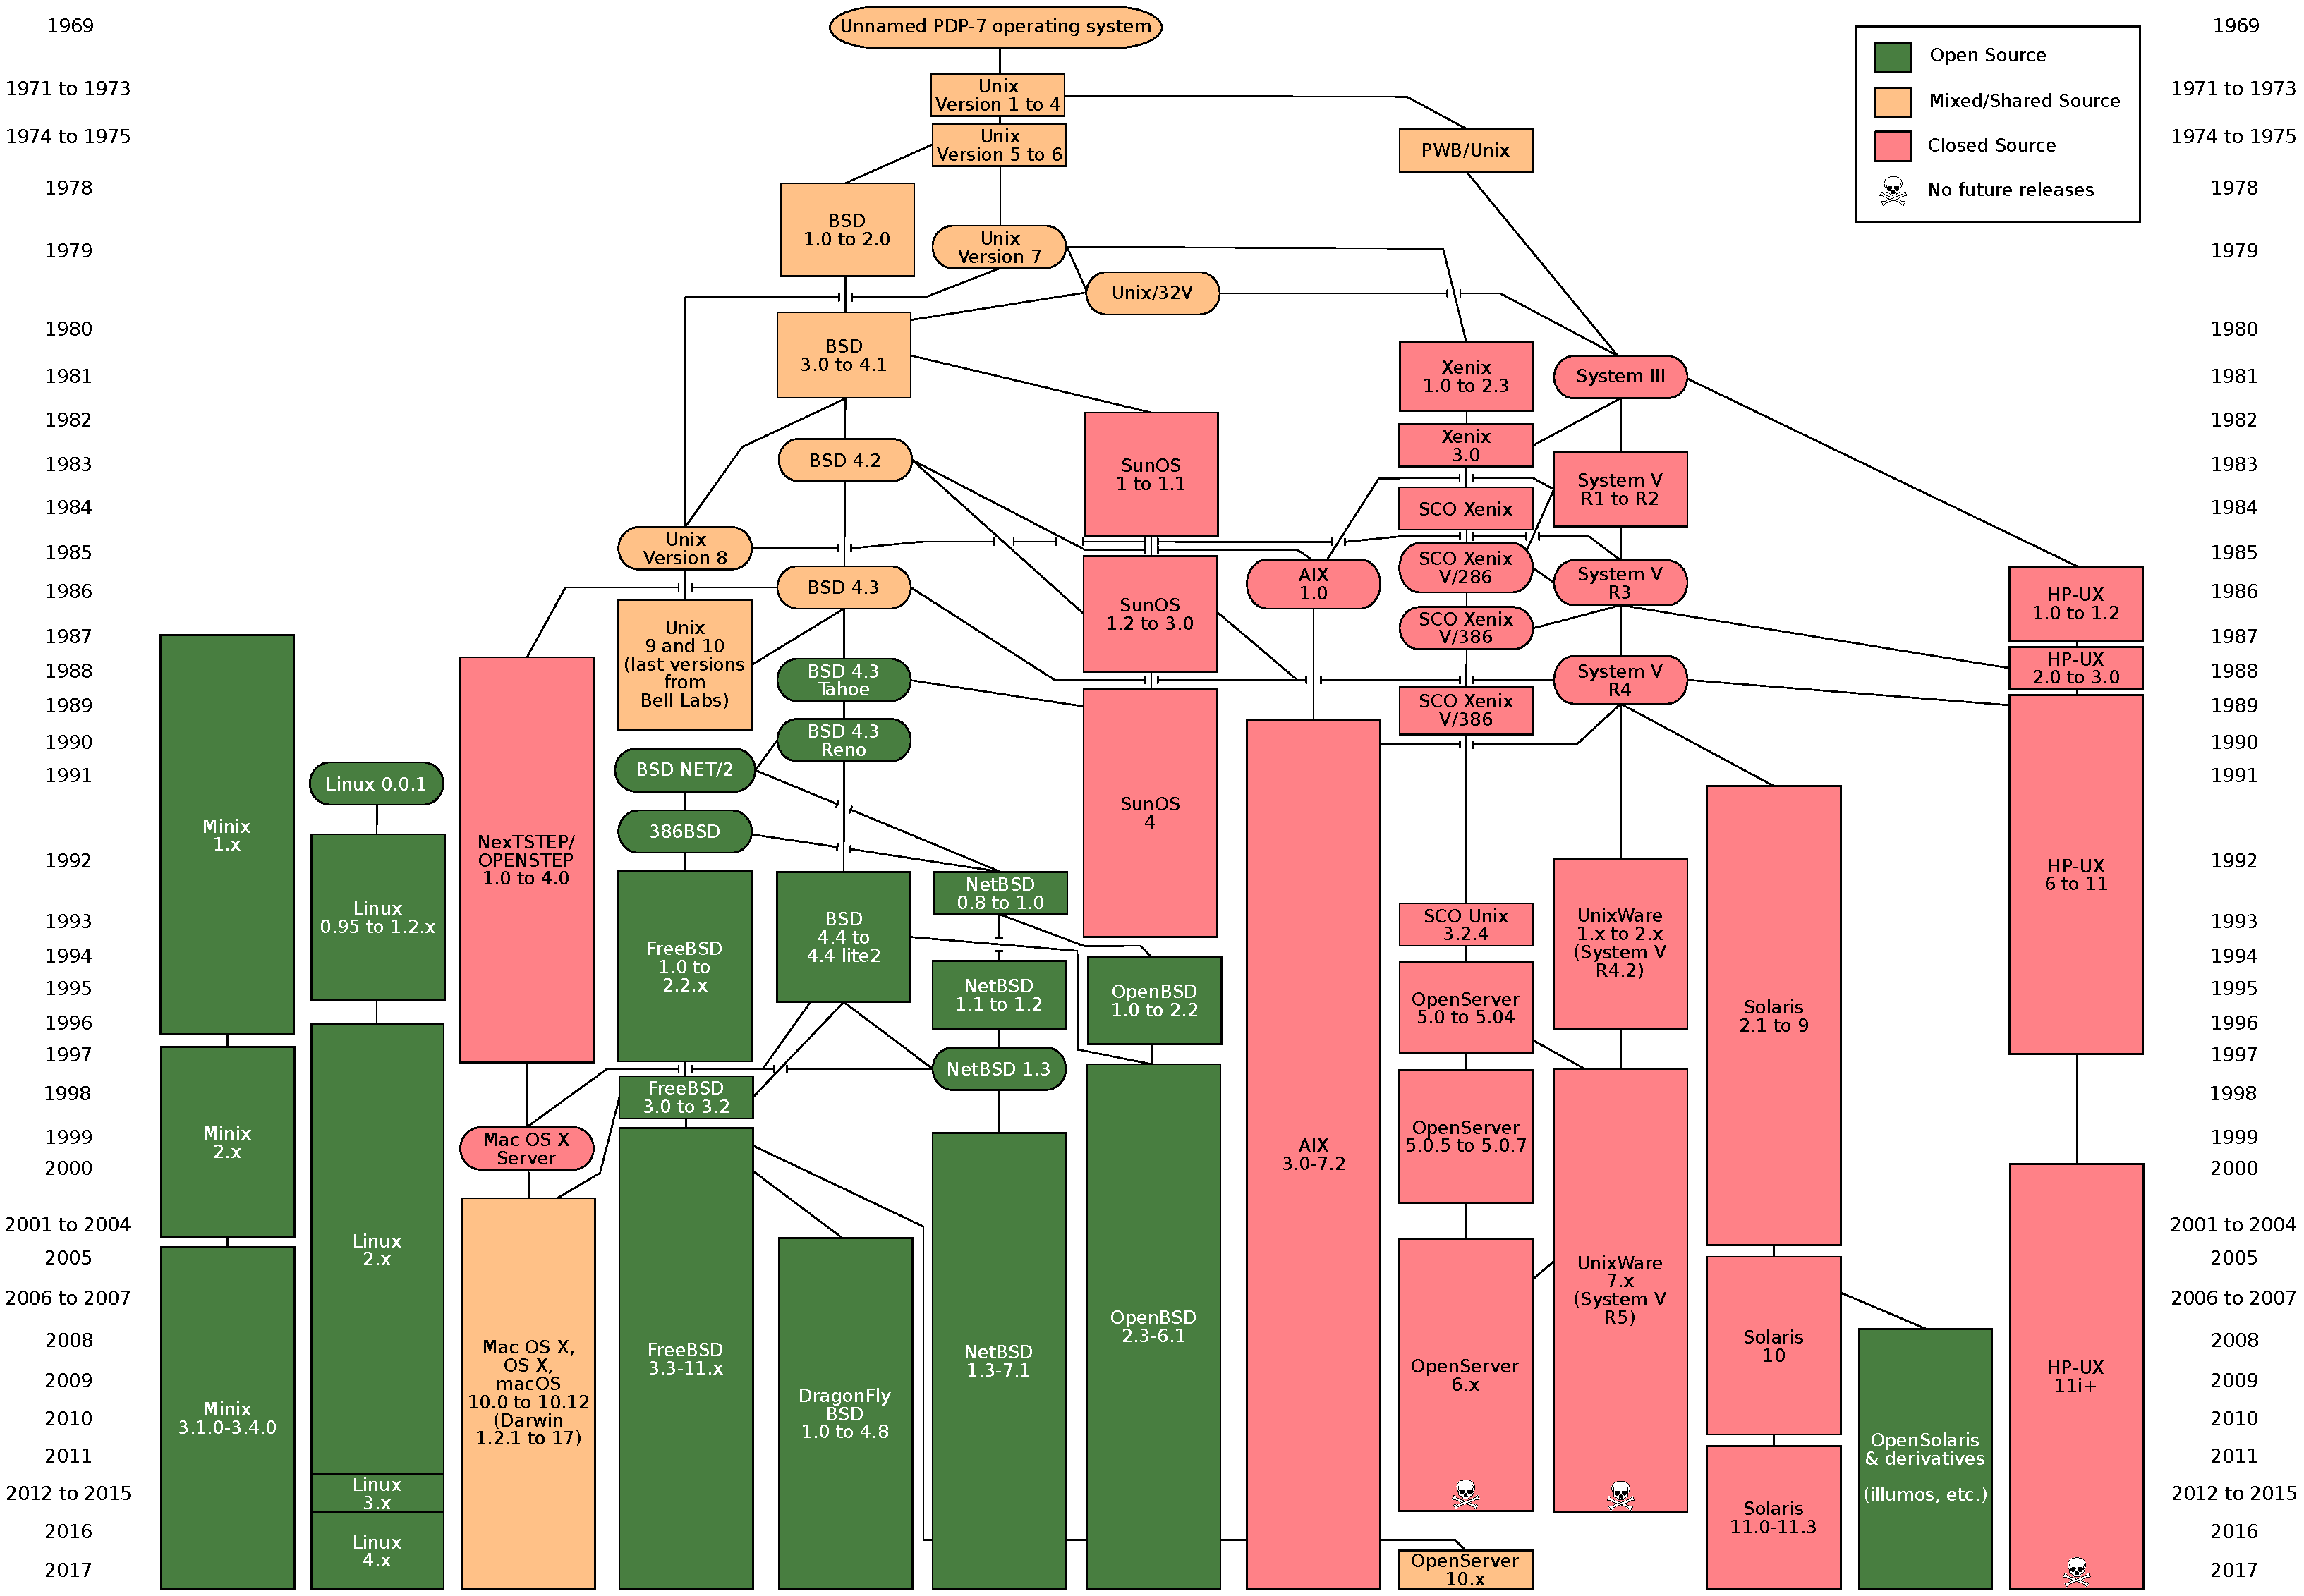
\includegraphics[height=0.9\textheight]{../unix-api/Unix_history-simple_en.pdf}
\imagecredit{image: Wikpedia/Eraserhead1+Infinity0+Sav\_vas}
\end{frame}

\begin{frame}{POSIX: standardized Unix}
\begin{itemize}
\item Portable Operating System Interface (POSIX) 
    \begin{itemize}
    \item ``standard for Unix''
    \end{itemize}
\item current version online: https://pubs.opengroup.org/onlinepubs/9699919799/
\item (almost) followed by most current Unix-like OSes
\item \ldots but OSes add extra features
\item \ldots and POSIX doesn't specify everything
\end{itemize}
\end{frame}

\begin{frame}{what POSIX defines}
\begin{itemize}
\item POSIX specifies the \myemph{library and shell interface}
    \begin{itemize}
    \item source code compatibility
    \end{itemize}
\item doesn't care what is/is not a system call\ldots
\item doesn't specify binary formats\ldots
\item idea: write applications for POSIX, recompile and run on all implementations
    \begin{itemize}
    \item this was a very important goal in the 80s/90s
    \item at the time, no dominant Unix-like OS (Linux was very immature)
    \end{itemize}
\end{itemize}
\end{frame}


\subsection{getpid}

\againframe<2>{posixProcessFunctions}

\begin{frame}[fragile,label=getpid]{getpid}
\begin{lstlisting}[language=C++]
pid_t my_pid = getpid();
printf("my pid is %ld\n", (long) my_pid);
\end{lstlisting}
\end{frame}

\begin{frame}[fragile,label=ps]{process ids in ps}
\begin{Verbatim}
cr4bd@machine:~$ ps
  PID TTY          TIME CMD
14777 pts/3    00:00:00 bash
14798 pts/3    00:00:00 ps
\end{Verbatim}
\end{frame}


\subsection{read, write}

% FIXME: work through examples more


\begin{frame}<0>[fragile,label=readWrite]{read/write}
\begin{lstlisting}
ssize_t read(int fd, void *buffer, size_t count);
ssize_t write(int fd, void *buffer, size_t count);
\end{lstlisting}
\begin{itemize}
\item read/write \myemph<2>{up to \textit{count}} bytes to/from \textit{buffer}
\item returns number of bytes read/written or -1 on error
    \begin{itemize}
    \item ssize\_t is a signed integer type
    \item error code in \texttt{errno}
    \end{itemize}
\item read returning 0 means end-of-file (\textit{not an error})
\begin{itemize}
\item can read/write less than requested (end of file, broken I/O device, \ldots)
\end{itemize}
\end{itemize}
\end{frame}

\againframe<1>{readWrite}

\begin{frame}[fragile,label=readExample1]{read'ing one byte at a time}
\begin{lstlisting}[language=C++,style=small,morekeywords=ssize\_t,morekeywords=string]
string s;
ssize_t amount_read;
char c;
/* cast to void * not needed in C */
while ((amount_read = read(STDIN_FILENO, (void*) &c, 1)) > 0) {
    /* amount_read must be exactly 1 */
    s += c;
}
if (amount_read == -1) {
    /* some error happened */
    perror("read"); /* print out a message about it */
} else if (amount_read == 0) {
    /* reached end of file */
}
\end{lstlisting}
\end{frame}



\begin{frame}[fragile,label=writeExample]{write example}
\begin{lstlisting}[language=C++,style=small]
/* cast to void * optional in C */
write(STDOUT_FILENO, (void *) "Hello, World!\n", 14);
\end{lstlisting}
\end{frame}



\section{partial reads and writes}
\againframe<2>{readWrite}
\subsection{partial reads and read error checking}

\begin{frame}[fragile,label=readExample2]{read'ing a fixed amount}
\begin{lstlisting}[language=C++,style=small,morekeywords=ssize\_t]
ssize_t offset = 0;
const ssize_t amount_to_read = 1024;
char result[amount_to_read];
do {
    /* cast to void * optional in C */
    ssize_t amount_read = 
        read(STDIN_FILENO,
             (void *) (result + offset),
             amount_to_read - offset);
    if (amount_read < 0) {
        perror("read"); /* print error message */
        ... /* abort??? */
    } else {
        offset += amount_read;
    }
} while (offset != amount_to_read && amount_read != 0);
\end{lstlisting}
\end{frame}

\begin{frame}{partial reads}
\begin{itemize}
    \item on regular file: read reads what you request
    \item but otherwise: usually gives you what's known to be available
        \begin{itemize}
            \item after waiting for something to be available
        \end{itemize}
    \vspace{.5cm}
    \item<2-> reading from network --- what's been received
    \item<2-> reading from keyboard --- what's been typed
\end{itemize}
\end{frame}

\subsection{partial writes and write error checking}

\begin{frame}[fragile,label=writeExampleErrorChecking]{write example (with error checking)}
\begin{lstlisting}[language=C++,style=small,morekeywords=ssize\_t]
const char *ptr = "Hello, World!\n";
ssize_t remaining = 14;
while (remaining > 0) {
    /* cast to void * optional in C */
    ssize_t amount_written = write(STDOUT_FILENO,
                                   ptr,
                                   remaining);
    if (amount_written < 0) {
        perror("write"); /* print error message */
        ... /* abort??? */
    } else {
        remaining -= amount_written;
        ptr += amount_written;
    }
}
\end{lstlisting}
\end{frame}

\begin{frame}{partial writes}
\begin{itemize}
    \item usually only happen on error or interruption
        \begin{itemize}
        \item but can request ``non-blocking''
        \item (interruption: via \textit{signal})
        \end{itemize}
    \item \textit{usually}: write \myemph{waits until it completes}
        \begin{itemize}
        \item = until remaining part fits in buffer in kernel
        \item does not mean data was sent on network, shown to user yet, etc.
        \end{itemize}
\end{itemize}
\end{frame}



\subsection{aside: environment variables}

\begin{frame}[fragile,label=envVarsPrintenv]{aside: environment variables (1)}
\begin{itemize}
\item key=value pairs associated with every process:
\end{itemize}
\begin{Verbatim}[fontsize=\fontsize{8}{9}\selectfont,commandchars=\\\{\}]
$ \textbf{printenv}
MODULE_VERSION_STACK=3.2.10
MANPATH=:/opt/puppetlabs/puppet/share/man
XDG_SESSION_ID=754
HOSTNAME=labsrv01 
SELINUX_ROLE_REQUESTED=
TERM=screen
SHELL=/bin/bash 
HISTSIZE=1000 
SSH_CLIENT=128.143.67.91 58432 22 
SELINUX_USE_CURRENT_RANGE=
QTDIR=/usr/lib64/qt-3.3
OLDPWD=/zf14/cr4bd
QTINC=/usr/lib64/qt-3.3/include
SSH_TTY=/dev/pts/0
QT_GRAPHICSSYSTEM_CHECKED=1
USER=cr4bd
LS_COLORS=rs=0:di=01;34:ln=01;36:mh=00:pi=40;33:so=01;35:do=01;35:bd=40;33;01:cd=40;33;01:or=40;31;01:mi=01;05;37;41:su=37;41:sg=30;43:ca=30;41:tw=30;42:ow=34;42:st=37;44:ex=01;32:*.tar=01;31:*.tgz=01;31:*.arc=01;31:*.arj=01;31:*.taz=01;31:*.lha=01;31:*.lz4=01;31:*.lzh=01;31:*.lzma=01;31:*.tlz=01;31:*.txz=01;31:*.tzo=01;31:*.t7z=01;31:*.zip=01;31:*.z=01;31:*.Z=01;31:*.dz=01;31:*.gz=01;31:*.lrz=01;31:*.lz=01;31:*.lzo=01;31:*.xz=01;31:*.bz2=01;31:*.bz=01;31:*.tbz=01;31:*.tbz2=01;31:*.tz=01;31:*.deb=01;31:*.rpm=01;31:*.jar=01;31:*.war=01;31:*.ear=01;31:*.sar=01;31:*.rar=01;31:*.alz=01;31:*.ace=01;31:*.zoo=01;31:*.cpio=01;31:*.7z=01;31:*.rz=01;31:*.cab=01;31:*.jpg=01;35:*.jpeg=01;35:*.gif=01;35:*.bmp=01;35:*.pbm=01;35:*.pgm=01;35:*.ppm=01;35:*.tga=01;35:*.xbm=01;35:*.xpm=01;35:*.tif=01;35:*.tiff=01;35:*.png=01;35:*.svg=01;35:*.svgz=01;35:*.mng=01;35:*.pcx=01;35:*.mov=01;35:*.mpg=01;35:*.mpeg=01;35:*.m2v=01;35:*.mkv=01;35:*.webm=01;35:*.ogm=01;35:*.mp4=01;35:*.m4v=01;35:*.mp4v=01;35:*.vob=01;35:*.qt=01;35:*.nuv=01;35:*.wmv=01;35:*.asf=01;35:*.rm=01;35:*.rmvb=01;35:*.flc=01;35:*.avi=01;35:*.fli=01;35:*.flv=01;35:*.gl=01;35:*.dl=01;35:*.xcf=01;35:*.xwd=01;35:*.yuv=01;35:*.cgm=01;35:*.emf=01;35:*.axv=01;35:*.anx=01;35:*.ogv=01;35:*.ogx=01;35:*.aac=01;36:*.au=01;36:*.flac=01;36:*.mid=01;36:*.midi=01;36:*.mka=01;36:*.mp3=01;36:*.mpc=01;36:*.ogg=01;36:*.ra=01;36:*.wav=01;36:*.axa=01;36:*.oga=01;36:*.spx=01;36:*.xspf=01;36:
MODULE_VERSION=3.2.10
MAIL=/var/spool/mail/cr4bd
PATH=/zf14/cr4bd/.cargo/bin:/zf14/cr4bd/bin:/usr/lib64/qt-3.3/bin:/usr/local/bin:/usr/bin:/usr/local/sbin:/usr/sbin:/opt/puppetlabs/bin:/usr/cs/contrib/bin:.
PWD=/zf14/cr4bd
LANG=en_US.UTF-8
MODULEPATH=/sw/centos/Modules/modulefiles:/sw/linux-any/Modules/modulefiles
LOADEDMODULES=
KDEDIRS=/usr
\textbf{\ldots}
_=/usr/bin/printenv
\end{Verbatim}
\end{frame}

\begin{frame}[fragile,label=envVarsFuncs]{aside: environment variables (2)}
\begin{itemize}
\item environment variable library functions:
    \begin{itemize}
    \item \texttt{getenv("KEY")} $\rightarrow$ \textit{value}
    \item \texttt{putenv("KEY=\textit{value}")} (sets KEY to \textit{value})
    \item \texttt{setenv("KEY", "value")} (sets KEY to \textit{value})
    \end{itemize}
\item {\fontsize{12}{13}\texttt{int execve(char *path, char **argv, char **envp)}}
\begin{lstlisting}[language=C++,style=small]
    char *envp[] = { "KEY1=value1", "KEY2=value2", NULL };
    char *argv[] = { "somecommand", "some arg", NULL };
    execve("/path/to/somecommand", argv, envp);
\end{lstlisting}
\item normal exec versions --- keep same environment variables
\end{itemize}
\end{frame}

\begin{frame}[fragile,label=envVarsUse]{aside: environment variables (3)}
\begin{itemize}
\item interpretation up to programs, but common ones\ldots
\vspace{.5cm}
\item \texttt{PATH=/bin:/usr/bin} 
    \begin{itemize}
    \item to run a program `foo', look for an executable in \texttt{/bin/foo}, then \texttt{/usr/bin/foo}
    \end{itemize}
\item \texttt{HOME=/zf14/cr4bd} 
    \begin{itemize}
    \item current user's home directory is `/zf14/cr4bd'
    \end{itemize}
\item \texttt{TERM=screen-256color} 
    \begin{itemize}
    \item your output goes to a `screen-256color'-style terminal
    \end{itemize}
\item \ldots
\end{itemize}
\end{frame}


\subsection{wait for mutliple}

\begin{frame}[fragile,label=typicalPatternMultiple1]{multiple processes?}
\begin{lstlisting}[language=C++,style=small]
while (...) {
    pid = fork();
    if (pid == 0) {
        exec ...
    } else if (pid > 0) {
        pids.push_back(pid);
    }
}

/* retrieve exit statuses in order */
for (pid_t pid : pids) {
    waitpid(pid, ...); 
    ...
}
\end{lstlisting}
\end{frame}
 

\subsection{wait for all}

\begin{frame}[fragile,label=waitForAny]{waiting for all children}
\begin{lstlisting}[
    language=C++,
    style=smaller,
    moredelim={**[is][\btHL<2|handout:0>]{@2}{2@}},
]
#include <sys/wait.h>
...
  while (true) {
    pid_t child_pid = waitpid(-1, &status, 0);
    if (child_pid == (pid_t) -1) {
      if (errno == ECHILD) {
        /* no child process to wait for */
        break;
      } else {
        /* some other error */
      }
    }
    /* handle child_pid exiting */
  }
\end{lstlisting}
\end{frame}


\subsection{wait for all (alt)}


\begin{frame}[fragile,label=typicalPatternMultiple2]{multiple processes?}
\begin{lstlisting}[language=C++,style=small]
while (...) {
    pid = fork();
    if (pid == 0) {
        exec ...
    } else if (pid > 0) {
        pids.push_back(pid);
    }
}

/* retrieve exit statuses as processes finish */
while ((pid = waitpid(-1, ...)) != -1) {
    handleProcessFinishing(pid);
}
\end{lstlisting}
\end{frame}



\subsection{waitpid WNOHANG}


\begin{frame}[fragile,label=waitNoHang]{`waiting' without waiting}
\begin{lstlisting}[
    language=C++,
    style=smaller,
    moredelim={**[is][\btHL<2|handout:0>]{@2}{2@}},
]
#include <sys/wait.h>
...
  pid_t return_value = waitpid(child_pid, &status, WNOHANG);
  if (return_value == (pid_t) 0) {
    /* child process not done yet */
  } else if (child_pid == (pid_t) -1) {
    /* error */
  } else {
    /* handle child_pid exiting */
  }
\end{lstlisting}
\end{frame}


\subsection{shell: background programs}

\begin{frame}[fragile,label=background]{running in background}
\begin{Verbatim}[fontsize=\small]
$ ./long_computation >tmp.txt &
[1] 4049
$ ...
[1]+    Done        ./long_computation > tmp.txt
$ cat tmp.txt
the result is ...
\end{Verbatim}
\begin{itemize}
\item \verb|&| --- run a program in ``background''
\item initially output PID (above: 4049)
\item print out after terminated
    \begin{itemize}
    \item one way: use \texttt{waitpid} with option saying ``don't wait''
    \end{itemize}
\end{itemize}
\end{frame}


\subsection{aside: on casting}

\begin{frame}[fragile,label=execvConst]{execv and const}
\begin{lstlisting}[language=C++,style=small]
int execv(const char *path, char *const *argv);
\end{lstlisting}
\begin{itemize}
    \item \texttt{argv} is a pointer to constant pointer to char
    \item probably should be a pointer to constant pointer to \textit{constant} char
    \item \ldots this causes some awkwardness:
\end{itemize}
\begin{lstlisting}[language=C++,style=small]
const char *array[] = { /* ... */ };
execv(path, array); // ERROR
\end{lstlisting}
    \begin{itemize}
    \item solution: cast
    \end{itemize}
\begin{lstlisting}[language=C++,style=small]
const char *array[] = { /* ... */ };
execv(path, (char **) array); // or (char * const *)
\end{lstlisting}
\end{frame}



\subsection{layers of file interfaces}

\usetikzlibrary{arrows.meta,chains}

\begin{frame}{layering}
\begin{tikzpicture}
\tikzset{
    box/.style={draw,thick,minimum width=8cm,minimum height=1cm},
    thin box/.style={fill=blue!20,minimum width=8cm,minimum height=1cm,outer sep=1mm},
}
\begin{scope}[start chain=going below,node distance=-.75mm,every node/.style={on chain}]
\node[box] (application) {application};
\node[box] (library) {standard library};
\node[thin box] (syscalls) {system calls};
\node[box] (kernel file) {kernel's file interface};
\node[box] (device driver) {device drivers};
\node[thin box] (hardware) {hardware interfaces};
\end{scope}
\draw[very thick] (kernel file.east) -- ++(1cm,0cm) node[right,font=\small] {kernel's buffers};
\draw[very thick] (syscalls.east) -- ++(1cm,0cm) node[right,font=\small] {read/write};
\draw[very thick] (library.east) -- ++(1cm,0cm) node[right,font=\small] {cout/printf --- \myemph{and their own buffers}};
\end{tikzpicture}
\end{frame}

\begin{frame}{why the extra layer}
    \begin{itemize}
        \item better (but more complex to implement) interface:
            \begin{itemize}
            \item read line 
            \item formatted input (scanf, cin into integer, etc.)
            \item formatted output
            \end{itemize}
        \item less system calls (bigger reads/writes) sometimes faster
            \begin{itemize}
            \item buffering can combine multiple in/out library calls into one system call
            \end{itemize}
        \item more portable interface
            \begin{itemize}
            \item cin, printf, etc. defined by C and C++ standards
            \end{itemize}
    \end{itemize}
\end{frame}


\subsection{parent and child}

\begin{frame}{parent and child processes}
\begin{itemize}
    \item every process (but process id 1) has a \textit{parent process} (\texttt{getppid()})
    \item this is the process that can wait for it
    \item creates tree of processes (Linux \texttt{pstree} command):
\end{itemize}
    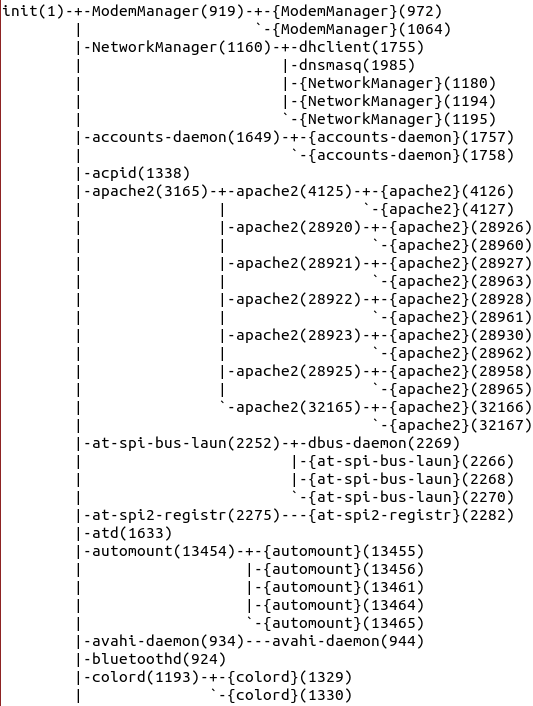
\includegraphics[height=0.6\textheight]{../unix-api/process-tree}
    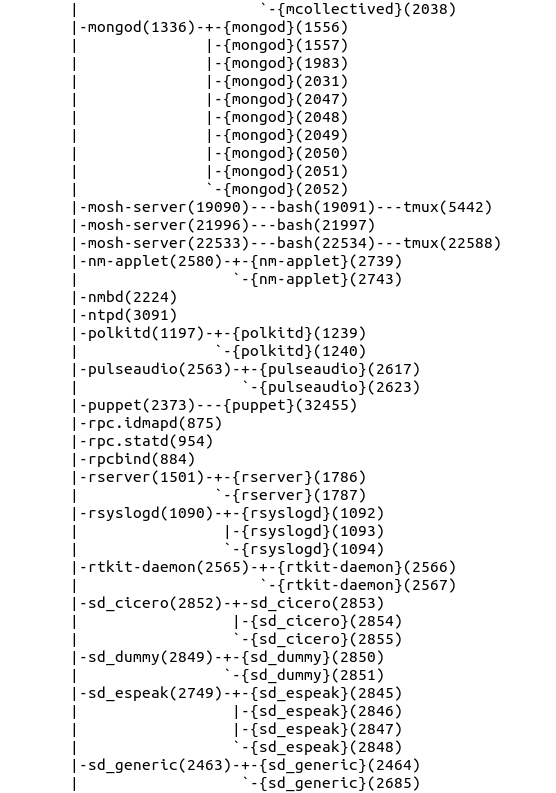
\includegraphics[height=0.6\textheight]{../unix-api/process-tree2}
\end{frame}

\begin{frame}{parent and child questions\ldots}
\begin{itemize}
    \item what if parent process exits before child?
        \begin{itemize}
        \item child's parent process becomes process id 1 (typically called \textit{init})
        \end{itemize}
    \item what if parent process never \texttt{waitpid()}s {\small (or equivalent)} for child?
        \begin{itemize}
        \item child process stays around as a ``zombie'' 
        \item can't reuse pid in case parent wants to use \texttt{waitpid()}
        \end{itemize}
    \item what if non-parent tries to \texttt{waitpid()} for child?
        \begin{itemize}
        \item waitpid fails
        \end{itemize}
\end{itemize}
\end{frame}


\subsection{kernel buffering}

\usetikzlibrary{arrows.meta,chains,shapes}

\begin{frame}{kernel buffering (reads)}
\begin{tikzpicture}
\tikzset{
    >=Latex,
    component box/.style={draw,thick,minimum width=10cm,minimum height=1cm,align=center},
    component box big/.style={component box,minimum height=2.5cm},
    component box small/.style={component box,minimum width=4cm},
    subcomponent box/.style={draw,thick,minimum width=2cm,align=center,font=\small},
    event line/.style={draw,ultra thick},
    event box/.style={draw,thick,fill=white,inner sep=0.25mm,font=\small, align=center},
    number box A/.style={draw=blue,thick,fill=blue!10,ellipse,font=\small,inner sep=0.1mm},
    number box A alt/.style={draw=blue,thick,dotted,fill=blue!5,ellipse,font=\small,inner sep=0.1mm,
            alt=<4>{draw=red,fill=red!10}},
    number box B/.style={draw=green,thick,fill=green!10,ellipse,font=\small,inner sep=0.1mm},
}
\node[component box] (process) {program};
\node[component box big,anchor=north] (os) at ([yshift=-2cm]process.south) {operating system \\ ~ \\ ~};
\node[component box small,anchor=north east] (keyboard) at ([xshift=-.5cm,yshift=-1.5cm]os.south) {keyboard};
\node[component box small,anchor=north west] (disk) at ([xshift=.5cm,yshift=-1.5cm]os.south) {disk};
\begin{visibleenv}<2->
\draw[event line,->] (keyboard.north) -- (os.south -| keyboard.north) node[midway,event box] (kp event){keypress happens, read};
\node[number box A,anchor=east] (kp event number) at (kp event.north west) {1};
\begin{visibleenv}<4->
    \node[number box A alt,anchor=east] at ([xshift=-.5cm,yshift=.1cm]kp event number.west) {2};
    \node[font=\small,anchor=east,inner sep=0.25mm] at (kp event number.west) {or};
\end{visibleenv}
\node[anchor=south,subcomponent box] (keyboard buffer)  at (os.south -| keyboard.north) {buffer: keyboard input \\ waiting for program};
\end{visibleenv}
\begin{visibleenv}<3->
    \draw[event line,->] ([xshift=-4cm]process.south) -- ([xshift=-4cm]os.north) node[midway,event box,xshift=-1cm] (read ev) {read char \\ from terminal};
\node[number box A,anchor=east] (read ev number) at (read ev.north west) {2};
\begin{visibleenv}<4->
    \node[number box A alt,anchor=east] at ([xshift=-.5cm,yshift=.1cm]read ev number.west) {1};
    \node[font=\small,anchor=east,inner sep=0.25mm] at (read ev number.west) {or};
\end{visibleenv}
    \draw[event line,<-] ([xshift=-2cm]process.south) -- ([xshift=-2cm]os.north) node[midway,event box,xshift=-.5cm] (from buf ev) {\ldots via buffer};
\node[number box A,anchor=east] at (from buf ev.north west) {3};
\end{visibleenv}
\begin{visibleenv}<5->
\draw[event line,->] ([xshift=1cm]process.south) -- ([xshift=1cm]os.north) node[midway,event box,xshift=0cm] (read file ev)  {read char \\ from file};
\node[number box B,anchor=east] at (read file ev.north west) {1};
\end{visibleenv}
\begin{visibleenv}<6->
\draw[event line,->] (disk.north) -- (os.south -| disk.north) node[midway,event box] (xfer disk ev) {read \textit{block} of data from disk};
\node[number box B,anchor=east] at (xfer disk ev.north west) {2};
\node[anchor=south,subcomponent box] at (os.south -| disk.north) {buffer: recently read \\ data from disk};
    \draw[event line,<-] ([xshift=4cm]process.south) -- ([xshift=4cm]os.north) node[midway,event box,xshift=0cm] (from disk buffer ev) {\ldots via buffer};
\node[number box B,anchor=east] at (from disk buffer ev.north west) {3};
\end{visibleenv}
\end{tikzpicture}
\end{frame}

\begin{frame}{kernel buffering (writes)}
\begin{tikzpicture}
\tikzset{
    >=Latex,
    component box/.style={draw,thick,minimum width=10cm,minimum height=1cm,align=center},
    component box big/.style={component box,minimum height=2.25cm},
    component box small/.style={component box,minimum width=4cm},
    subcomponent box/.style={draw,thick,minimum width=2cm,align=center,font=\small},
    event line/.style={draw,ultra thick},
    event box/.style={draw,thick,fill=white,inner sep=0.25mm,font=\small, align=center},
}
\node[component box] (process) {program};
\node[component box big,anchor=north] (os) at ([yshift=-2cm]process.south) {operating system \\ ~ \\ ~};
\node[component box small,anchor=north east] (network) at ([xshift=-.5cm,yshift=-1.5cm]os.south) {network};
\node[component box small,anchor=north west] (disk) at ([xshift=.5cm,yshift=-1.5cm]os.south) {disk};
\begin{visibleenv}<3->
\draw[event line,<-] (keyboard.north) -- (os.south -| keyboard.north) node[midway,event box] {(when ready) \\ send data};
\node[anchor=south,subcomponent box] (keyboard buffer)  at (os.south -| keyboard.north) {buffer: output \\ waiting for network};
\end{visibleenv}
\begin{visibleenv}<2->
\draw[event line,->] ([xshift=-4cm]process.south) -- ([xshift=-4cm]os.north) node[midway,event box,xshift=0cm] {print char \\ to remote machine};
\end{visibleenv}
\begin{visibleenv}<4->
\draw[event line,->] ([xshift=1cm]process.south) -- ([xshift=1cm]os.north) node[midway,event box,xshift=0cm] {write char \\ to file};
\end{visibleenv}
\begin{visibleenv}<5->
\draw[event line,<-] (disk.north) -- (os.south -| disk.north) node[midway,event box] {(when ready) \\ write \textit{block} of data from disk};
\node[anchor=south,subcomponent box] at (os.south -| disk.north) {buffer: data waiting \\ to be written on disk};
\end{visibleenv}
\end{tikzpicture}
\end{frame}

\begin{frame}{read/write operations}
\begin{itemize}
\item read()/write(): move data into/out of buffer
\item possibly wait if buffer is empty (read)/full (write)
\vspace{.5cm}
\item actual I/O operations --- wait for device to be ready
    \begin{itemize}
    \item trigger process to stop waiting if needed
    \end{itemize}
\end{itemize}
\end{frame}


\subsection{open}

\begin{frame}{filesystem abstraction}
\begin{itemize}
\item regular files --- named collection of bytes
    \begin{itemize}
    \item also: size, modification time, owner, access control info, \ldots
    \end{itemize}
\item directories --- folders containing files and directories
    \begin{itemize}
    \item hierarchical naming: \texttt{/net/zf14/cr4bd/fall2018/cs4414}
    \item \textit{mostly} contains regular files or directories
    \end{itemize}
\end{itemize}
\end{frame}

\begin{frame}[fragile,label=openExample]{open}
\begin{lstlisting}[
    language=C++,
    moredelim={**[is][\btHL<1-|handout:1->]{@1}{1@}},
]
int open(const char *path, int flags);
int open(const char *path, int flags, int mode);
...

int read_fd = open("dir/file1", O_RDONLY);
int write_fd = open("/other/file2",
        O_WRONLY | O_CREAT | O_TRUNC, 0666);
int rdwr_fd = open("file3", O_RDWR);
\end{lstlisting}
\end{frame}

\begin{frame}[fragile,label=openExplainPath]{open}
\begin{lstlisting}[
    language=C++,
    moredelim={**[is][\btHL<1-|handout:1->]{@1}{1@}},
]
int open(const char *@1path1@, int flags);
int open(const char *@1path1@, int flags, int mode);
\end{lstlisting}
\begin{itemize}
\item path = filename
\item e.g. \texttt{"/foo/bar/file.txt"}
    \begin{itemize}
    \item \texttt{file.txt} in 
    \item directory \texttt{bar} in
    \item directory \texttt{foo} in 
    \item ``the root directory''
    \end{itemize}
\item e.g. \texttt{"quux/other.txt}
    \begin{itemize}
    \item \texttt{other.txt} in 
    \item directory \texttt{quux} in
    \item ``the current working directory'' (set with \texttt{chdir()})
    \end{itemize}
\end{itemize}
\end{frame}

\begin{frame}[fragile,label=openExplainFDs]{open: file descriptors}
\begin{lstlisting}[
    language=C++,
    moredelim={**[is][\btHL<1-|handout:1->]{@1}{1@}},
]
@1int1@ open(const char *path, int flags);
@1int1@ open(const char *path, int flags, int mode);
\end{lstlisting}
\begin{itemize}
\item return value = \myemph{file descriptor} {\small (or -1 on error)}
\item index into table of \textit{open file descriptions} for each process
\item used by system calls that deal with open files
\end{itemize}
\end{frame}



\subsection{Unix: everything is a file}

\usetikzlibrary{arrows.meta,chains}

\begin{frame}{POSIX: everything is a file}
\begin{itemize}
\item the file: one interface for
    \begin{itemize}
    \item devices (terminals, printers, \ldots)
    \item regular files on disk
    \item networking (sockets)
    \item local interprocess communication (pipes, sockets)
    \end{itemize}
    \vspace{.5cm}
    \item basic operations: open(), read(), write(), close()
\end{itemize}
\end{frame}


\section{pipe exercise (partial reads)}


\begin{frame}<1>[fragile,label=pipeExtraEx2]{exercise}
\vspace{-.25cm}
\begin{lstlisting}[language=C++,basicstyle=\tt\fontsize{9.5}{10.5}\selectfont]
int pipe_fds[2]; pipe(pipe_fds);
pid_t p = fork();
if (p == 0) {
  close(pipe_fds[0]);
  for (int i = 0; i < 10; ++i) {
    char c = '0' + i;
    write(pipe_fds[1], &c, 1);
  }
  exit(0);
}
close(pipe_fds[1]);
char buffer[10];
ssize_t count = read(pipe_fds[0], buffer, 10);
for (int i = 0; i < count; ++i) {
  printf("%c", buffer[i]);
}
\end{lstlisting}
Which of these are possible outputs {\small (if pipe, read, write, fork don't fail)}?
\begin{tabular}{lll}
A. \texttt{0123456789} & B. \texttt{0} & C. (nothing) \\
\myemph<2>{D.} A and B & E. A and C & F. A, B, and C \\
\end{tabular}
\end{frame}

\iftoggle{heldback}{}{\againframe<2>{pipeExtraEx2}}

\begin{frame}<0>[fragile,label=pipeExtraEx2More]{empirical evidence}
\begin{Verbatim}
      8 0
    374 01
    210 012
     30 0123
     12 01234
      3 012345
      1 0123456
      2 01234567
      1 012345678
    359 0123456789
\end{Verbatim}
\end{frame}

\iftoggle{heldback}{}{\againframe<2>{pipeExtraEx2More}}

\begin{frame}{partial reads}
\begin{itemize}
\item read returning 0 always means end-of-file
    \begin{itemize}
    \item by default, read always waits \textit{if no input available yet}
    \item but can set read to return \textit{error} instead of waiting
    \end{itemize}
\item read can return less than requested if not available
    \begin{itemize}
        \item e.g. child hasn't gotten far enough
    \end{itemize}
\end{itemize}
\end{frame}
 % FIXME: cut?

\section{pipe: closing?}
\begin{frame}{pipe: closing?}
    \begin{itemize}
    \item if all write ends of pipe are closed
        \begin{itemize}
        \item can get end-of-file (read() returning 0) on read end
        \item exit()ing closes them
        \end{itemize}
    \item $\rightarrow$ close write end when not using
    \vspace{.5cm}
    \item generally: limited number of file descriptors per process
    \item $\rightarrow$ good habit to close file descriptors not being used
    \item (but probably didn't matter for read end of pipes in example)
    \end{itemize}
\end{frame}


\subsection{pipe exercise}

\begin{frame}[fragile,label=pipeExtraEx1]{exercise}
\begin{lstlisting}[language=C++,basicstyle=\tt\fontsize{9.5}{10.5}\selectfont]
pid_t p = fork();
int pipe_fds[2];
pipe(pipe_fds);
if (p == 0) { /* child */
  close(pipe_fds[0]);
  char c = 'A';
  write(pipe_fds[1], &c, 1);
  exit(0);
} else { /* parent */
  close(pipe_fds[1]);
  char c;
  int count = read(pipe_fds[0], &c, 1);
  printf("read %d bytes\n", count);
}
\end{lstlisting}
The child is trying to send the character \texttt{A} to the parent, but
the above code outputs \texttt{read 0 bytes} instead of \texttt{read 1 bytes}.
What happened?
\end{frame}

\begin{frame}{exercise solution}
    \begin{itemize}
        \item \iftoggle{heldback}{~}{pipe() is after fork --- two pipes, one in child, one in parent}
    \end{itemize}
\end{frame}

 % FIXME: formatting

\subsection{pipe example}

\begin{frame}[fragile,label=pipeExample]{pipe example (1)}
\begin{lstlisting}[
    language=C++,
    style=smaller,
    moredelim={**[is][\btHL<2|handout:0>]{@2}{2@}},
    moredelim={**[is][\btHL<3|handout:2>]{@3}{3@}},
    moredelim={**[is][\btHL<4|handout:3>]{@4}{4@}},
]
int pipe_fd[2];
if (pipe(pipe_fd) < 0)
    handle_error(); /* e.g. out of file descriptors */
int read_fd = pipe_fd[0];
int write_fd = pipe_fd[1];
@2child_pid = fork();2@
@2if (child_pid  == 0) {2@
    /* in child process, write to pipe */
    @4close(read_fd);4@
    write_to_pipe(write_fd); /* function not shown */
    exit(EXIT_SUCCESS);
@2} else if (child_pid > 0) {2@
    /* in parent process, read from pipe */
    @3close(write_fd);3@
    read_from_pipe(read_fd); /* function not shown */
    @2waitpid(child_pid, NULL, 0);2@
    @4close(read_fd);4@
} @2else {2@ /* fork error */ }
\end{lstlisting}
\begin{tikzpicture}[overlay,remember picture]
\coordinate (box place) at ([xshift=-1cm,yshift=-1cm]current page.north east);
\tikzset{
    box/.style={draw=red,thick,fill=white,anchor=north east,at={(box place)},align=left,font=\small},
}
\begin{visibleenv}<2|handout:0>
\node[box] {
    `standard' pattern with fork()
};
\end{visibleenv}
\begin{visibleenv}<3|handout:2>
\node[box] {
    read() will not indicate \\
    end-of-file if write fd is open  \\
    (any copy of it)
};
\end{visibleenv}
\begin{visibleenv}<4|handout:3>
\node[box] {
    have habit of closing \\
    to avoid `leaking' file descriptors \\
    you can run out
};
\end{visibleenv}
\end{tikzpicture}
\end{frame}

